\chapter{Conceptual Deductive Analysis}
\label{Conceptual Deductive Analysis}

The structure of the \ac{CDA}, as previously described in the \nameref{methodology} section, is as follows:
The relevant concepts of the three main paradigms to be integrated will be introduced first.
While going from the general to the specific and attempting to give both an overview of the broader topic
as well as a detailed understanding of the specific aspects that are relevant to our research.

Based on the knowledge gained and presented thereby,
the hypothetical model will be developed of how these paradigms may be integrated and what implications this may have.

% Conceptual Deductive Analysis about Cloud Computing
\section{Cloud Computing}
\label{sec:Cloud_Computing}

Outsourcing IT infrastructure and services to third parties,
rather than maintaining them in-house, has gained popularity as a cost-effective and flexible solution for businesses.
It allows for reduced upfront costs and increased scalability. \footcite{armbrustCloudsBerkeleyView}

It has become especially popular in form of multi tenant data centers, which are able to provide services to many customers.
This ability to share the costs burden of the infrastructure amongst their customers, making use of the economies of scale
has lead to the rise of the three main cloud providers, Amazon Web Services, Microsoft Azure and Google Cloud Platform\footcite{InfographicAmazonMaintains2024}.

These multi tenant data centers need to guarantee the isolation of hardware and software resources between the different customers,
as highly sensitive, valuable, and mission critical data is stored and processed in these data centers.

While this need has existed before the advent of the cloud computing business model,
as user isolation is a fundamental requirement of any multi-user system,
the need for isolation has become more important since number of customers and the amount of data stored and processed has increased significantly.
This has led to the continual development of virtualization and containerization technologies,
which are used to provide the necessary isolation between the different customers\footcite{randalIdealRealRevisiting2021}.

The two main technologies used to provide these isolated environments are virtualization and containerization.
What they are and how they work will be discussed in the following sections.

\subsection{Virtualization and Isolation}
\label{sec:virtualization}

The differentiating factor of \ac{VM}s is that they are at their core hardware emulators.
They consist of a \gls{host} \ac{OS}, a so called hypervisor and one or more \gls{guest} \ac{OS},
including their dedicated virtual resources like \ac{CPU}, memory, storage, and network interfaces\footcite{gotoKernelbasedVirtualMachine2011}.

This does not only provide isolation between the processes running on the different \gls{guest} \ac{OS}s,
but also enables the users and developers to emulate hardware architectures and run different \ac{OS}s than the \gls{host} \ac{OS}


In figure \ref{fig:full_virtualization} the different layers of a full virtualization setup are shown.
The hardware layer is the actual hardware, which is used to run the \ac{OS} and the hypervisor.

The Hypervisor is a software layer which is responsible for the management of the different \ac{VM}s,
while it may be a separate piece of software, it can also be tightly integrated into the \ac{OS} itself
and is then called a type 1 hypervisor, while a hypervisor running on top of an \ac{OS} is called a type 2 hypervisor\footcite{awsTypeVsType}.

\begin{figure}[ht!]
    \vspace{0.5cm}
    \centering
    \scalebox{0.75}{
        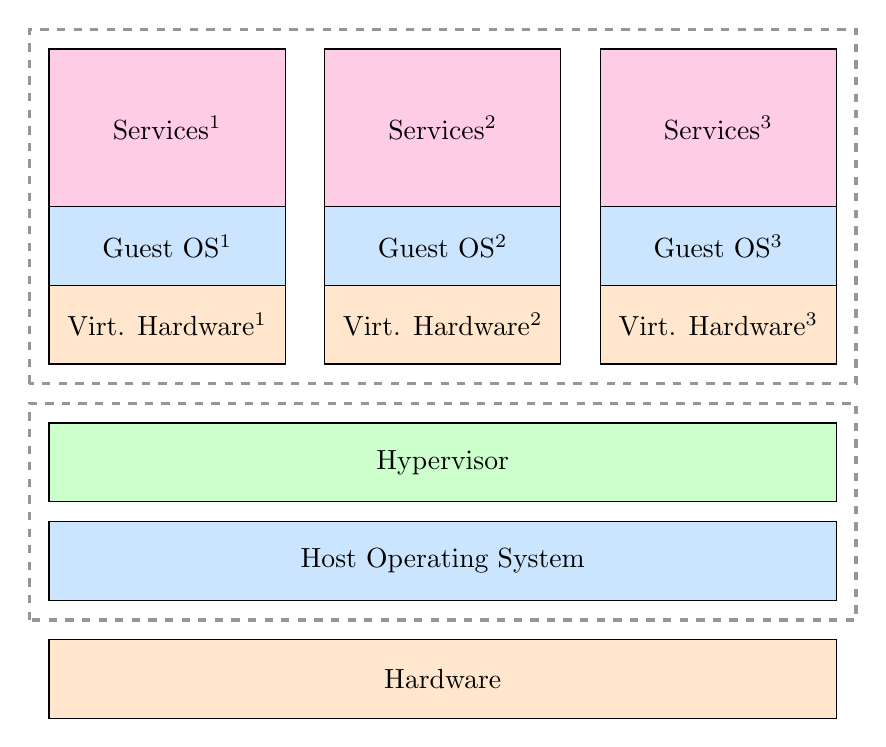
\begin{tikzpicture}
            % Define the colors
            \definecolor{hardwarecolor}{RGB}{255, 230, 204}
            \definecolor{oscolor}{RGB}{204, 229, 255}
            \definecolor{hypervisorcolor}{RGB}{204, 255, 204}
            \definecolor{vmcolor}{RGB}{255, 204, 229}
            \definecolor{dashedlinecolor}{RGB}{150, 150, 150}

            % Draw the Hardware layer
            \filldraw[fill=hardwarecolor, draw=black] (0,0) rectangle (10,1) node[pos=.5] {Hardware};

            % Draw the Host Operating System layer
            \filldraw[fill=oscolor, draw=black] (0,1.5) rectangle (10,2.5) node[pos=.5] {Host Operating System};

            % Draw the Hypervisor layer
            \filldraw[fill=hypervisorcolor, draw=black] (0,2.75) rectangle (10, 3.75) node[pos=.5] {Hypervisor};

            % Draw the dashed boundary of the Host and Hypervisor
            \draw[dashed, draw=dashedlinecolor, very thick] (-0.25,1.25) rectangle (10.25,4.0);

            % Draw the Virtual Machines layer
            % VM1
            \filldraw[fill=hardwarecolor, draw=black] (0, 4.5) rectangle (3, 5.5) node[pos=.5] {Virt. Hardware\textsuperscript{1}};
            \filldraw[fill=oscolor, draw=black] (0, 5.5) rectangle (3, 6.5) node[pos=.5] {Guest OS\textsuperscript{1}};
            \filldraw[fill=vmcolor, draw=black] (0, 6.5) rectangle (3, 8.5) node[pos=.5] {Services\textsuperscript{1}};
            % VM2
            \filldraw[fill=hardwarecolor, draw=black] (3.5, 4.5) rectangle (6.5, 5.5) node[pos=.5] {Virt. Hardware\textsuperscript{2}};
            \filldraw[fill=oscolor, draw=black] (3.5, 5.5) rectangle (6.5, 6.5) node[pos=.5] {Guest OS\textsuperscript{2}};
            \filldraw[fill=vmcolor, draw=black] (3.5, 6.5) rectangle (6.5, 8.5) node[pos=.5] {Services\textsuperscript{2}};
            % VM3
            \filldraw[fill=hardwarecolor, draw=black] (7, 4.5) rectangle (10, 5.5) node[pos=.5] {Virt. Hardware\textsuperscript{3}};
            \filldraw[fill=oscolor, draw=black] (7, 5.5) rectangle (10, 6.5) node[pos=.5] {Guest OS\textsuperscript{3}};
            \filldraw[fill=vmcolor, draw=black] (7, 6.5) rectangle (10, 8.5) node[pos=.5] {Services\textsuperscript{3}};

            % Draw the dashed boundary of the Virtual Machines
            \draw[dashed, draw=dashedlinecolor, very thick] (-0.25,4.25) rectangle (10.25,8.75);

        \end{tikzpicture}
    }
    \caption{Full Virtualization}
    \label{fig:full_virtualization}
\end{figure}

While virtualization is a powerful tool, it is not without its drawbacks, as the overhead of the emulation of an entire hardware stack is a significant performance hit,
which is why \ac{KVM} and Xen have been developed. They are able to pass through instructions directly to \gls{host}s hardware.

Features like \gls{VT-d}, \gls{virtio} and \gls{EPT} are used to respectively pass through \ac{CPU} instructions, network/storage interfaces and memory management to the hardware,
if the hardware supports these features.
But if the hardware does not support these features, the hypervisor will fall back to emulate the needed hardware making it support a wider range of hardware,
but at the cost of performance\footcite{barhamXenArtVirtualization2003}.


\subsection{Containerization}
\label{sec:containerization}

With the need for isolated environments and the economic desire for a more efficient use of resources,
the next logical step was to create a solution which trades the flexibility of virtualization for the
performance of executing \ac{CPU} instructions native to the \gls{host} hardware\footcite{ercegAnotherBriefHistory2022}.

This gap was gradually filled by the development of containerization technologies in the Linux kernel,
by way of giving the \gls{host} \ac{OS} the ability to “jail” processes and denying them to interact with other processes and the \gls{host} \ac{OS}.
This enables the \gls{host} \ac{OS} to run multiple isolated environments, which are called containers,
with close to native performance. \footcite{randalIdealRealRevisiting2021}

The downside of this approach is the strong dependency on the \gls{host}s kernel,
which means that all the containers are bound to its architecture and may not use features of newer kernels,
or legacy features of older kernels\footcite{kovacsComparisonDifferentLinux2017}.

\begin{figure}[ht!]
    \vspace{0.5cm}
    \centering
    \scalebox{0.75}{
        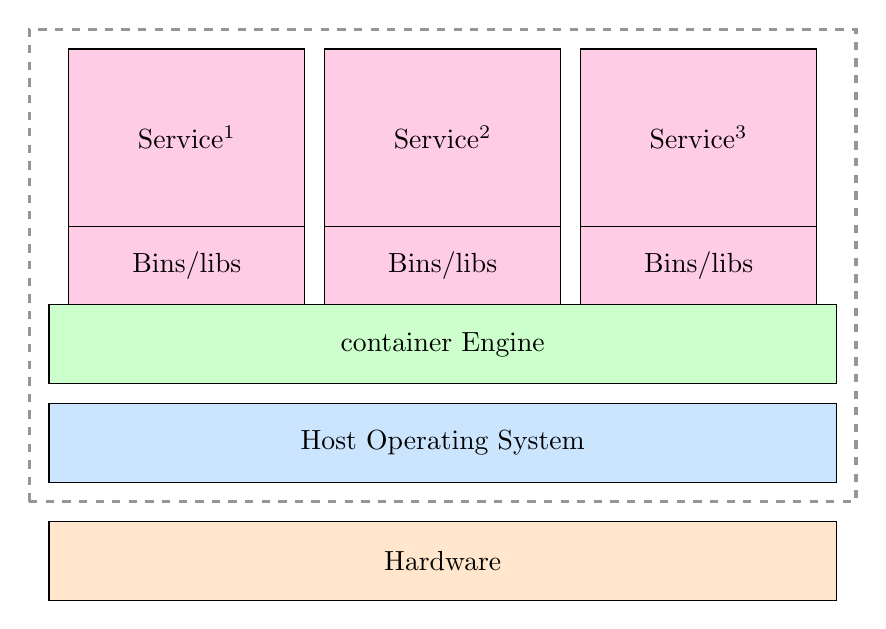
\begin{tikzpicture}
            % Define the colors
            \definecolor{hardwarecolor}{RGB}{255, 230, 204}
            \definecolor{oscolor}{RGB}{204, 229, 255}
            \definecolor{hypervisorcolor}{RGB}{204, 255, 204}
            \definecolor{containercolor}{RGB}{255, 204, 229}
            \definecolor{dashedlinecolor}{RGB}{150, 150, 150}

            % \definecolor{hardwarecolor}{RGB}{217, 224, 189} % Pale yellow
            % \definecolor{oscolor}{RGB}{236, 219, 230} % Lavender
            % \definecolor{hypervisorcolor}{RGB}{185, 218, 247} % Light blue
            % \definecolor{containercolor}{RGB}{204, 247, 220} % Light green
            % \definecolor{dashedlinecolor}{RGB}{255, 235, 204} % Light orange

            % Draw the Hardware layer
            \filldraw[fill=hardwarecolor, draw=black] (0,0) rectangle (10,1) node[pos=.5] {Hardware};

            % Draw the Host Operating System layer
            \filldraw[fill=oscolor, draw=black] (0,1.5) rectangle (10,2.5) node[pos=.5] {Host Operating System};

            % Draw the container Engine layer
            \filldraw[fill=hypervisorcolor, draw=black] (0,2.75) rectangle (10, 3.75) node[pos=.5] {container Engine};

            % Draw the containers layer
            % container1
            \filldraw[fill=containercolor, draw=black] (0.25,  3.75) rectangle (3.25,  4.75) node[pos=.5] {Bins/libs};
            \filldraw[fill=containercolor, draw=black] (0.25,  4.75) rectangle (3.25, 7) node[pos=.5] {Service\textsuperscript{1}};
            % container2
            \filldraw[fill=containercolor, draw=black] (3.5,  3.75) rectangle (6.5,  4.75) node[pos=.5] {Bins/libs};
            \filldraw[fill=containercolor, draw=black] (3.5,  4.75) rectangle (6.5, 7) node[pos=.5] {Service\textsuperscript{2}};
            % container3
            \filldraw[fill=containercolor, draw=black] (6.75,  3.75) rectangle (9.75,  4.75) node[pos=.5] {Bins/libs};
            \filldraw[fill=containercolor, draw=black] (6.75,  4.75) rectangle (9.75, 7) node[pos=.5] {Service\textsuperscript{3}};
            % Draw the dashed boundary of the Host and containers
            \draw[dashed, draw=dashedlinecolor, very thick] (-0.25,1.25) rectangle (10.25,7.25);

        \end{tikzpicture}
    }
    \caption{Containerization}
    \label{fig:containerization}
\end{figure}

In figure \ref{fig:containerization}, a containerization setup is depicted, which includes the hardware,
the \gls{host} \ac{OS}, and the container engine.
The container engine is responsible for managing the containers and the resources they use as well as providing a unified way to interact with the containers.

The emergence of containerization was more of a gradual process than a single release of a new technology,
but the three most important steps in this process were the introduction of the chroot system call,
the introduction of namespaces and the introduction of c-groups, which will be discussed in the following sections.

\subsubsection{Chroot}

The first major step towards process isolation was the introduction of the chroot system call in the 7th edition of Unix and later in the 4.0BSD release,
which was further developed to the chroot jail
These jails where used as am security tool to protect the larger system in \textit{BSD},
this sentiment was not applied when Linux adopted the chroot system call\footcite{bernsteinContainersCloudLXC2014}

While not technically being considered a security feature, as it was not designed to be inherently secure, and therefore is easy to circumvent\footcite{linux-manualpageChrootLinuxManual},
it does provide a way to isolate processes from the rest of the system.
As changing the \gls{root_fs} directory of a process and its children to an arbitrary directory, results in them considering this directory as the \gls{root_fs} of the file system.

This prevents a given process effectively from reaching outside this boundary, as it is unable to access files outside the new \gls{root_fs} directory.
Linux works under the paradigm  "everything is a file”, which means that everything on the system is represented within the file system,
be it a process, a network interface or a block device.
So if the process is unable to access the file, it is unable to access the resource.
This is useful for running untested code which is not suspected to be actively malicious, or for providing a restricted environment for a process to run in.

While some consider \textit{chroot} the first step towards containerization, some argue \footcite{randalIdealRealRevisiting2021} that the true origin might be attributed to the  “process capabilities” function,
which allowed for the limitation of process resource utilization and permissions, this is a key feature of containerization, but as they fell out of favor after the advent of virtualization, we will not discuss them further.

\subsubsection{Namespaces}

The central feature of isolation in modern Linux containerization beyond the simple separation of the file system is the use of namespaces.

As the \textit{chroot} command only provides a way to deny access sections of the file system, a process still needs some way to interact with the rest of the system,
for example to access the network or to create new processes it would need access to the \texttt{/proc} file system, undercutting the isolation provided by chroot.
Therefore, a way to provide a process with its own segregated view of the system is needed, which is where namespaces come in\footcite{datadogContainerSecurityFundamentals2023}

Namespaces are a feature of the Linux kernel, which is used to provide isolation between the 6 different classes of kernel resources.
Five of which are so-called privileged namespaces, which require \gls{root_priv} access to create and manage\footcite{217614}.

\pagebreak

The five privileged namespaces are:
\begin{itemize}
    \item \textbf{PID} — Process IDs
    \item \textbf{NET} — Network devices, stacks, ports, etc.
    \item \textbf{IPC} — System V IPC, POSIX message queues
    \item \textbf{MNT} — Mount points
    \item \textbf{UTS} — Hostname and NIS domain name
\end{itemize}

The sixth namespace, the \textbf{User} namespace, is special,
because it can be used by unprivileged users to create containers,
which is not possible with the other namespaces\footcite{priedhorskyCharliecloudUnprivilegedContainers2017}.

Namespaces are applied to all Linux processes, regardless of whether they run in a container or not,
every process has its own view of the system, which is demarcated by the ID of the namespace it is running in.
Processes with the same namespace ID share the same view of the system,
while processes' with different namespaces are totally ignorant of the other processes existence and influence on the system\footcite{michaelkerriskNamespacesOperationPart2013}.


% I already spent way too much time on this graph!!
% todo: Dont touch ever again!!! 

\begin{figure}[!ht]
    \centering
    \vspace{0.5cm}
    \scalebox{0.75}{
        \begin{tikzpicture}[
                every node/.style = {
                        shape=circle,
                        draw,
                        align=center,
                        minimum size=10mm,
                        inner sep=1pt,
                    },
                level/.style={sibling distance=50mm/#1},
                note/.style={rectangle, draw=none, align=left},
                nsnode/.style={circle, draw, align=center, minimum size=10mm, inner sep=1pt}
            ]


            \node[label=right:init] {1}
            child { node {2}
                    child { node (10) [nsnode] {\textcolor{red}{1}(\textcolor{darkgray}{10})}
                            child { node (11) [nsnode] {\textcolor{red}{2}(\textcolor{darkgray}{11})}}
                            child { node (12) [nsnode] {\textcolor{red}{3}(\textcolor{darkgray}{12})}
                                    child { node (13) [nsnode] {\textcolor{red}{4}(\textcolor{darkgray}{13})}}
                                }
                        }
                }
            child { node {3}
                    child { node {4}}
                    child { node {5}
                            child { node (6) [nsnode] {\textcolor{red}{1}(\textcolor{darkgray}{6})}
                                    child {node (7) [nsnode] {\textcolor{red}{2}(\textcolor{darkgray}{7})}}
                                    child {node (8) [nsnode] {\textcolor{red}{3}(\textcolor{darkgray}{8})}
                                            child {node (9) [nsnode] {\textcolor{red}{4}(\textcolor{darkgray}{9})}}
                                        }
                                }
                        }
                };

            \node[draw=red,fit=(6) (7) (8) (9), inner sep=8pt, label={[rotate=90, anchor=south, yshift=-18mm]west:\color{red}Nested PID Namespace}, shape=rectangle] {};

            \node[draw=red,fit=(10) (11) (12) (13), inner sep=8pt, label={[rotate=90, anchor=south, yshift=-16mm]west:\color{red}Nested PID Namespace}, shape=rectangle] {};

        \end{tikzpicture}
    }
    \caption{Namespace isolation\protect\footnotemark}
    \label{fig:pid_namespace_isolation}
\end{figure}
\footnotetext{Modified from \cite{sultanContainerSecurityIssues2019}}


In figure \ref{fig:pid_namespace_isolation} a simple example of the \ac{PID} namespace is shown,
where the processes 1, 2, 3, 4 and 5 are running in the “init” namespace, which is the namespace the \gls{host} \ac{OS} is running in.
The processes 6, 7, 8 and 9 are running in their own nested \ac{PID} namespace, believing to be the only processes on the system.
The same goes for the processes 10, 11, 12 and 13, which also believe to be processes 1, 2, 3 and 4 in their own namespaces.
This results in a hierarchy of namespaces, where the parents are able to see the children, but not the other way around.
So if a process in the “init” namespace were to kill process 1, it would identify it with its true ID of 1 addressing it in the “init” namespace.
But if it wanted to kill within the nested namespace, it can reference the processed with ID 1 of the namespace by using the ID 6
as the internal \ac{PID}s of a namespace are mapped to a different \ac{PID} in the parents namespace\footcite{michaelkerriskNamespacesOperationPart2013}.

\subsubsection{Control groups}
\label{sec:control_groups}

While chroot isolates the file system and namespaces isolate system resources,
a given service might think it is alone on the system and starts to take up all the resources it can get,
filling memory, taking up all the \ac{CPU} time and saturating the network.
To prevent this from happening intentionally or unintentionally, control groups were introduced \footcite{dockerCgroupsNamespacesWhat2015}
for each of the namespaces, so that each process can be limited in all 6 dimensions.

The c-groups have two levels of enforcement for the limitations,
on one hand there is the hard limit, which is an absolute limit,
that if exceeded will result in the process being terminated immediately.
On the other hand there is also the soft limit which lets the process exceed the limit for a certain amount of time.
But if the system is starved for resources, the services which are overstepping the most get killed first\footcite{linuxkernel-docsMemoryResourceController}.

% Interesting side node,
% how do the c-groups enfroce the limitations?
% Cpu limtiations arent done via percentage but core
% If the memory is exeeded there are two enforcement levels,
% either the process is terminated immedatly,
% or, if the system is running out iof memory, the services which are overstepping the most get killed first.
% 
% additionaly its not possible not to use c groups and namespaces, 
% as they are so deeply ingraned in the way the modern linux works.
% therefore not performance can be gained by not running something in a contianer.

% \subsusbsecton{Union Capable File Systems}
% If more pages are needed for the paper, this could be a good topic to expand on.


\subsubsection{Capabilities}

While the namespaces limit what can be seen and interacted with,
and the c-groups limit how much of the resources can be used,
the \textit{capabilities} make sure that the processes are not able to do anything they are not supposed to do.

This need comes from the binary way Linux handles permissions, as either \gls{root_priv} or not \gls{root_priv}.
In the context of containers we need to differentiate between the ultimate power a process may exert within its own namespace,
but the fine-grained control over what a process may modify in the \gls{host} system.

An example for this would be to \gls{host} an Apache server in a container,
in order to expose the web server to the internet, the container needs to be able to bind to a port.
Without \textit{capabilities} feature the container would need to run as \gls{root_priv}, which would pose a security risk,
as the container would be able to do anything the \gls{root_priv} user can do, which is not desirable.

This is where \textit{capabilities} come in.
They are a way to give a process a subset of the \gls{root_priv} users capabilities,
which are needed to perform a certain task, without giving it the full power of the \gls{root_priv} user.

In the case of the Apache server, the process would need the capability to bind to a port, which is the \texttt{CAP\_NET\_BIND\_SERVICE} capability.
\footcite{sultanContainerSecurityIssues2019}



% what happens when a container is started?

% diagram:
% Docker Daemon
% clone( CLONE_NEWIPC | CLONE_NEWNET |
% CLONE_NEW\ac{PID} | CLONE_NEWUTS | CLONE_NEWNEWNS)
% \gls{host}name setup
% rootfs setup
% pivot root
% mount /dev, /proc, /sys
% IP, firewall setup
% execve( Apache2 )

\pagebreak

\subsection{Container Runtimes}

All these major features work to enable the concept of containers,
the coordination of these features is done via the container runtime
which is responsible for the creation, management, and destruction of containers.

\subsubsection{LXC}

The first container runtime was \ac{LXC}, which was developed in 2008 by the Linux kernel community\footcite{jordanwebbLXCLXDDifferent},
it was the first to exclusively use the mainline kernel features to provide isolation and centered around the idea of a “system container”,
a container pretending to be a full \ac{OS}, which is able to run multiple services and applications\footcite{kumarans.PracticalLXCLXD2017}.

\subsubsection{Docker}
\label{sec:docker}
Nowadays, one of the most popular container runtimes is Docker - a high-level container runtime \footcite{vailsheryLeadingContainerizationTechnologies}
focusing on “application containers”, which are used to run a singular service per container.
Docker extends the basis of  \ac{LXC} container runtime by a \ac{AUFS} file system,
as well as further kernel features providing further isolation\footcite{debabContainersRuntimesWar2021}.

The whole Docker project aims to provide a simple and easy to use interface to the underlying containerization technologies,
it administrates the containers through a unified \ac{API}, the docker \gls{daemon}, to which and from where all the communication goes.

It also provides a standard way of predefining environments, by way of the docker image format.
The docker consists of a set of immutable \ac{RO} layers, stacked onto of each other and then combined with a \ac{COW} layer,
these combine to the file system of the container runtime.
While the \ac{RO} layers are shared between different containers and instances, as resources.
the \ac{COW} layer is unique to each container and is used to store the changes made to the file system for this container\footcite{morabitoHypervisorsVsLightweight2015}.

While Docker has become the de facto standard for containerization, it is not without its drawbacks,
as the docker daemon mandates \gls{root_priv} access to run and operate.
This has been considered as undesirable in the \ac{HPC} community\footcite{mujkanovicSurveyAdaptiveContainerization2023} and some consider it to be proving too large of an attack surface\footcite{priedhorskyCharliecloudUnprivilegedContainers2017}.
Several alternatives have been developed, some as a drop-in replacement for the Docker runtime
like \ac{CRI-O} and Podman, while others like Singularity and Charliecloud are designed to be used in the \ac{HPC} community specifically.


% \subsubsection{Singularity}
% does not require root access to run containers, which is a big plus for \ac{HPC} systems, because the administrators are not always willing to give root access to the users.
% if one wants to run root comands in the container one needs to have the root access on the \gls{host} system, which is a big plus for security.
% has its own MPI support, supports infiniband, gpu and excellerator support
% \footcite{priedhorskyCharliecloudUnprivilegedcontainers2017}
% "here are several pminent issues with this approach, the first being compatibility.
%  The software makes use of kernel namespaces that are not deemed stable by multiple prominent distributions of Linux (e.g. no versions of Red Hat Enterprise Linux or compatibles support it), 
% and may not be included in these distributions for the foreseeable future.
%  A closely related issue is one of dependencies" \footcite{kurtzerSingularityScientificcontainers2017}

\subsection{Orchestration}
\label{sec:orchestration}

For now, we have only talked about the creation and management of containers in the scope of a single \gls{host},
but as the containerization effort was driven by Googles need to manage their data centers,
It was always the intention to manage containers in a distributed environment\footcite{vermaLargescaleClusterManagement2015}.

Coordinating the execution, communication and scheduling of containers in a large scale environment is called orchestration,
and has become a key feature for the cloud computing business model, as it allows for a more efficient use of resources than virtualization
and a more secure and flexible way than traditional \ac{HPC} \glsplural{batch system}\footcite{kennyKubernetesHPCAdministration2021} which will be discussed in the \ref{sec:CDA_HPC} section.

The three dominating orchestrations are Kubernetes, Docker Swarm and Mesos,
with Kubernetes being the most popular by a wide margin, with 46\% of companies reporting to use at least one Kubernetes based service
while Swarm and Mesos are used by 11\% and 9\% of companies respectively\footcite{gardenContainerOrchestratorUsage}.
All these tools have a significant feature overlap,
while differing in their internal approach\footcite{truyenComprehensiveFeatureComparison2019}.
As Kubernetes is by far the most popular while having the most in common with the other two,
we will be using it as a reference for the following discussion.

Kubernetes works as a distributed declarative system,
that means that instead of being told what to do, it is told what should be,
and the cluster does its best to make the desired state a reality.


\subsubsection{Kubernetes Basic Concepts}


At the heart of Kubernetes are the \textit{pods}, they are the smallest deployable unit in Kubernetes
and consist of one or more containers, which are always running together as a single unit.

As they share the same namespaces for network and storage, they are able to communicate with each other and share data.
So even the components of Kubernetes itself are containers running as pods on the cluster.
The core functionality of Kubernetes is to manage and schedule these pods on the different \gls{Node}s of the cluster
and to provide them with the necessary resources to run.

The way to interface with the cluster is through providing a \textit{manifest}, a description of a desired state of the cluster,
usually in form of a \acs{YAML} file, which is then submitted to the \textit{API server} of the cluster.
These manifests specify in which way and under which conditions the pods should be running on the cluster,
and the \textit{controller manager} of the cluster is responsible for making sure that the desired state is a reality.

There are several types of controllers which are used, but the most important of which are the \textit{Jobs}, the \textit{Deployments}, \textit{StatefulSets} and \textit{DaemonSets}.


\begin{itemize}
    \item \textbf{Jobs} are one off tasks which are run to completion, similar to a \gls{batch system} job in a \ac{HPC} environment.
    \item \textbf{Deployments} are used to declare a state of the cluster,
          for example that at anytime there should be 3 instances of a web server running, no matter what happens.
    \item \textbf{StatefulSets} as all the containers in the pods are ephemeral, they will not persist their state after they are terminated,
          for this reason a StatefulSet can be used to provide a stable network identity and stable storage for which an instance of a pod can be associated with.
    \item \textbf{DaemonSets} are pods which permanently run on the nodes of the cluster,
          they are used to provide additional interfaces between the clusters nodes and the containers running on them e.g. a network proxy or a monitoring agent.
\end{itemize}

\subsubsection{High Level architecture}
To ensure a controllable environment for the containers to run in and to communicate with each other, a homogeneous substrate
is provided across the different nodes of the cluster, which is the responsibility of the \textit{container runtime} and the \textit{container network interface}.
To keep all these nodes in sync and to provide a unified way to interact with the cluster, the \textit{control plane} which is itself a containers on the cluster.
The high level architecture of Kubernetes is divided into two main parts, the control plane and the nodes,
The control plane is responsible for the coordination of the different nodes and the management of the different resources.
Itself is divided into several \gls{mico-service} like components, which are responsible for the different management tasks.
Just like everything else the services of the containers themselves are containers running on the cluster\footcite{kubernetes-docsKubernetesComponents}.
The cluster may consist of a single node or thousands of nodes, which are responsible for the actual execution of the containers\footcite{kubernetes-docsNodes}.


\begin{figure}[!ht]
    \centering
    \vspace{0.5cm}
    \scalebox{0.85}{
        \begin{tikzpicture}[node distance=1cm and 1.5cm]
            % Commands to change color scheme

            \definecolor{etcdcolor}{RGB}{237, 240, 177} 1
            \definecolor{controlplanecolor}{RGB}{255, 204, 229}
            \definecolor{nodecolor}{RGB}{204, 229, 255}
            \definecolor{clientcolor}{RGB}{204, 255, 204}
            \definecolor{CNIcolor}{RGB}{255, 230, 204}

            \def\nbetcd{3}
            \def\nbapiserver{2}
            \def\nbscheduler{2}
            \def\nbcontroller{2}
            \def\nbnode{3}
            \edef\alletcd{}
            \foreach \i in {1,...,\nbetcd}{
                    \node[draw, fill=etcdcolor] at ($ (360/\nbetcd * \i:0.9) $) (etcd\i) {etcd};
                    \xdef\alletcd{(etcd\i) \alletcd}
                }
            \node[draw,dotted, fit=\alletcd, inner sep=2mm] (etcd) {};

            \foreach \i in {1,...,\nbscheduler}{
                    \node[draw,
                        rotate fit=90,
                        left=of etcd,
                        fill=controlplanecolor,
                        fit=(etcd.north west) (etcd.south west),
                        minimum height=0.7cm,
                        xshift=\i mm,
                        yshift=-\i mm] (scheduler\i) {};
                }
            \node[draw=none, align=center,rotate=90] at (scheduler\nbscheduler) {scheduler};

            \foreach \i in {1,...,\nbcontroller}{
                    \node[draw,
                        rotate fit=90,
                        left=3cm of scheduler1,
                        fill=controlplanecolor,
                        fit=(etcd.north west) (etcd.south west),
                        minimum height=0.7cm,
                        xshift=\i mm,
                        yshift=-\i mm] (controller\i) {};
                }
            \node[align=center,rotate=90] at (controller\nbcontroller) {controller};

            \foreach \i in {1,...,\nbapiserver}{
                    \node[draw,
                        above=of etcd,
                        fill=controlplanecolor,
                        fit=(scheduler1.north east) (controller1.north east) (etcd.north east),
                        minimum height=0.7cm,
                        xshift=\i mm,
                        yshift=\i mm] (apiserver\i) {};
                }
            \node[align=center] at (apiserver\nbapiserver) {apiserver};
            \draw[<->] (etcd.north) -- (etcd.north|-apiserver1.south);


            \node[above right=5cm of apiserver\nbapiserver] (kubelet1) {};
            \foreach \i in {1,...,\nbnode}{
                    \node[draw, fill=controlplanecolor] (kubelet-box\i) at (kubelet\i) {kubelet};
                    \node[draw,below=0.4cm of kubelet\i, fill=CNIcolor] (runtime\i) {runtime};
                    \node[draw,left=0.2cm of runtime\i, fill=controlplanecolor] (proxy\i) {proxy};
                    \node[draw,right=0.2cm of runtime\i, fill=CNIcolor] (CNI\i) {CNI};
                    \node[draw,below=0.9cm of runtime\i,
                        fit=(runtime\i) (CNI\i) (proxy\i),
                        inner sep=0mm, fill=nodecolor] (kernel\i) {};
                    \node[align=center] at (kernel\i) {kernel};
                    \draw[->] (kubelet-box\i) -- (runtime\i.north);
                    \draw[->] (runtime\i) -- (runtime\i|-kernel\i.north);
                    \draw[<-] (CNI\i) -- (CNI\i |- kernel\i.north);
                    \draw[->] (proxy\i) -- (proxy\i |- kernel\i.north);
                    \node[draw,
                        dashed,
                        fit=(kubelet\i) (runtime\i) (CNI\i) (kernel\i),
                        inner sep=2mm,
                        label={\scriptsize{node\i}}]  (node\i) {};
                    \draw[->] (kubelet-box\i.west) -- ++(-2.25cm,0) |- (apiserver\nbapiserver.east);
                    \draw[-] (proxy\i.north) -- ++(0, 0.55);

                    \pgfmathtruncatemacro\nextnode{\i+1}
                    \node[draw=none, below=2.9cm of kubelet\i] (kubelet\nextnode) {};
                }

            \draw[<->] (scheduler\nbscheduler.east) -- (scheduler\nbscheduler.east|-apiserver1.south);
            \draw[<->] (controller\nbscheduler.east) -- (controller\nbscheduler.east|-apiserver1.south);

            \node[draw,
                dashed,
                fit=(etcd) (apiserver1) (apiserver\nbapiserver),
                inner sep=2mm] (controlplane-nodes) {};

            \node[draw,
                above=1cm of apiserver\nbapiserver,
                minimum width=3cm,
                minimum height=0.7cm,
                fill=clientcolor] (client) {Client};
            \draw[<->] (client) -- (apiserver\nbapiserver);

            \coordinate (Start) at ($(CNI1.east)+(0.7cm,0)$);
            \coordinate (End) at ($(CNI\nbnode.east)+(0.7cm,0)$);

            \foreach \i in {1,...,\nbnode}
                {
                    \ifnum\i<\nbnode
                        \pgfmathtruncatemacro\nextNode{\i+1}
                        \draw ($(CNI\i.east)$) -- +(+0.7cm,0) -|  ($(CNI\nextNode.east)+(0.7cm,0)$) -- ($(CNI\nextNode.east)$);
                    \fi
                }

            % Label for the CNI network
            \path (Start) -- (End) node[midway, anchor=south, rotate=-90] {Node-Network};

            %% Stop  using the tikz, you always get lost in the details and never get anything done.
            %% Its just too much fun to play with the details.
        \end{tikzpicture}
    }
    \caption{High Level Architecture\protect\footnotemark}
    \label{fig:high_level_architecture}
\end{figure}

\footnotetext{Modified from \cite{zempashiZempashiKubetraining}}


\textbf{Control Plane}

A state is declared to the system via the unified \ac{API} \texttt{kube-apiserver},
this preferred state is then given to the \texttt{etcd}, a distributed \gls{kv store},
which is used as the \gls{Single source of truth} for the cluster\footcite{nalawalaComprehensiveStudyEtcd2022}.

On a regular basis, the \texttt{kube-controller-manager} checks the actual state of the cluster against the desired state,
if the actual state deviates form the desired state\footcite{kubernetes-docsCloudControllerManager}
the \linebreak
\texttt{kube-controller-manager} will wake the corresponding controller for the resource in question,
which knows what to do to make the actual state match the desired state \footcite{kubernetes-docsControllers}

This woken controller then submits a request to the \texttt{kube-scheduler} via the \ac{API},
which then assigns the task to a node, based on the current scheduling policy\footcite{kubernetes-docsKubernetesScheduler}.

\textbf{Nodes}

On the Side of the clusters nodes, the \texttt{kubelet} is responsible for interfacing with the local container runtime
through the \ac{CRI} and handles the execution of the containers locally on behest of the larger cluster.
Once the kubelet has announced itself to the \texttt{kube-apiserver} the node is ready to run containers.
If the scheduler has assigned a task to the node, the \texttt{kubelet} will check if it
needs to pull the container image from the registry, and then start the container\footcite{kubernetes-docsKubelet}.

The other service running on all nodes is the \ac{CNI}, which is responsible for the networking of the containers.
The \ac{CNI} is a plugin-based system, which allows for the use of different underlying networking solutions,
in order to provide the container with a layer 3 network interfaces and a \ac{IP} address\footcite{thelinuxfoundationCNI}.

The \texttt{kube-proxy} is responsible for regularly checking in with the \texttt{kube-apiserver} and updating the local \ac{IP} tables,
to make sure that the containers are able to communicate with each other and the outside world\footcite{kubernetes-docsKubeproxy}.

The containers themselves are run within a \texttt{Pod}, which is the smallest unit of work in Kubernetes.
While a \texttt{Pod} can consist of as little as a  singular container, the idea is to provide a way to allocate a main container,
in combination with additional supporting containers, which are used to provide additional services to the main container.
An example for this would be a main container running a service which needs to be able to access a database.

The connection to the \ac{DB} instead of hard-coding the service simply calls localhost,
and the support container being a sidecar container, which is working as an easily replaceable proxy to the database.

All this while a third container captures the entire stdout and stderr of the main container and sends it to a log aggregator.

\subsubsection{Networking}
\label{sec:K8sNetworking}

As already mentioned the networking of Kubernetes is quite involved in order to provide the flexibility, isolation, and performance needed for a large scale distributed system.
This is because the containers need to be replaceable on a whim, accessible both from the outside and the inside of the cluster,
but should also all have a unique \ac{IP} address without the need for \gls{NAT}.
This is achieved by abstracting the networking into three different levels, the pod level, the node level and the cluster level.


\begin{figure}[!ht]
    \centering
    \scalebox{0.85}{
        \begin{tikzpicture}[node distance=1cm and 1.5cm]
            \definecolor{nodecolor}{RGB}{204, 229, 255}
            \definecolor{servicenetworkcolor}{RGB}{255, 204, 229}
            \def\nbnode{3} % Number of nodes

            % Assuming a maximum number of pods to calculate node sizes dynamically
            \def\maxpods{3}
            \def\podsize{1cm}


            % Define styles for elements
            \tikzset{
                nodebox/.style={draw, fill=nodecolor, minimum width=3.5cm, minimum height=5cm},
                pod/.style={inner sep=0pt, minimum size=\podsize}
            }

            \foreach \i in {1,...,\nbnode}{
                    % Draw nodes
                    \node[nodebox] (node\i) at (5*\i, 0) {};
                    \node[above=0 of node\i] {Node \i};

                    % Dynamically calculate the number of pods for this example
                    % \pgfmathtruncatemacro\nbpods{random(2,\maxpods)}
                    \pgfmathtruncatemacro\nbpods{\maxpods}

                    % Calculate starting xshift to center pods
                    \pgfmathsetmacro\startxshift{(\podsize - \nbpods*1cm) / 2 - 0.25cm}



                    % Draw pods inside each node equally spaced on the x-axis and centered
                    \foreach \j in {1,...,\nbpods}{
                            % Adjust xshift for each pod
                            \pgfmathsetmacro\currentxshift{\startxshift + (\j-1)*1cm}
                            \node[pod, right=of node\i.west, xshift=\currentxshift, yshift=-1cm] (pod\i\j) {
\includegraphics[width=\podsize,height=\podsize]{graphics/k8s_pod.png}};

                        }
                }

            % Sercice network box
            \fill[draw,dashed, fill=servicenetworkcolor, opacity=0.5] ($(node1.north west)+(0.25,-0.25)$) rectangle ($(node\nbnode.mid east)+(-0.25,0)$);

            % Drawing to paralel lines in the the service network box the same length as the pod network line
            \draw ($(node1.north west)+(0.5,-1)$) -- ($(node\nbnode.north east)+(-0.5,-1)$) ;
            \draw ($(node1.north west)+(0.5,-2)$) -- ($(node\nbnode.north east)+(-0.5,-2)$) ;

            \node at ($(node2.north)+(0,-0.75)$) {Service Networks};


            % Draw the node network line dynamically based on nodes
            \coordinate (Start) at ($(node1.south west)+(-0.5cm,-1cm)$);
            \coordinate (End) at ($(node\nbnode.south east)+(0.5cm,-1cm)$);
            \draw (Start) -- (End) node[midway,below] {Node Network};

            % Draw lines from the middle of the nodes to the node network
            \foreach \i in {1,...,\nbnode}{
                    \draw (node\i.south) -- ($(node\i.south)+(0,-1cm)$);
                }

            % Draw the pod network line dynamically based on pods
            \coordinate (PodStart) at ($(pod11.south west)+(0, -0.5cm)$);
            \coordinate (PodEnd) at ($(pod\nbnode\maxpods.south east)+(0,-0.5cm)$);
            \draw (PodStart) -- (PodEnd) node[midway,below] {Pod Network};

            % Draw lines from the bottom of each pod to the pod network
            \foreach \i in {1,...,\nbnode}{
                    \foreach \j in {1,...,\maxpods}{
                            \draw (pod\i\j.south) -- ($(pod\i\j.south)+(0,-0.5cm)$);

                            % Randomly decide whether the pod connects to service network line 1, line 2, or none
                            \pgfmathsetmacro\connectTo{int(random(0,2))} % Generates 0, 1, or 2

                            % Connect to service network line 1
                            \ifnum\connectTo=1
                                \draw (pod\i\j.north) -- ($(pod\i\j.north)+(0,1cm)$);
                            \fi

                            % Connect to service network line 2
                            \ifnum\connectTo=2
                                \draw (pod\i\j.north) -- ($(pod\i\j.north)+(0,2cm)$);
                            \fi
                            % If \connectTo is 0, no line is drawn
                        }
                }

            % Draw encompassing box for the k8s cluster
            \node[draw, dashed, fit=(node1) (node\nbnode) (Start) (End), inner sep=1cm, label=above:Kubernetes Cluster] (cluster) {};

        \end{tikzpicture}
    }
    \caption{Kubernetes Network Diagram\protect\footnotemark}
    \label{abb: k8s_networkdiagramm}
\end{figure}
\footnotetext{Based on: \cite{kubernetes-docsClusterNetworkinga}}


\textbf{Pod level}
At the pod level, the containers share the same network namespace and therefore also the same \ac{IP} address.
The communication between the different containers happens through the loop-back interface,
so that the containers are able to communicate with each by simply calling on their \texttt{localhost} interface.
This is made possible through the \texttt{pause} container, a container in every pod which handles the whole administration
of basic tasks, like  setup  of the namespaces, network interfaces or the killing of \gls{zombies} in the \ac{PID} namespace\footcite{sookocheffGuideKubernetesNetworking2018}.

\textbf{Node level}

Each pod has its own network namespace and its own dedicated \ac{IP} address, which is unique to the pod and is reachable from the entire cluster.
If two pods need to communicate with each other,
each of them \gls{patching} their network interface to the root network namespace via a \texttt{\ac{VETH}} pair.
Now the root network namespace can see the two \texttt{\ac{VETH}} endpoints as two network interfaces,
it can \gls{bridge}  the two interfaces, which allows the two pods to communicate with each other \footcite{sookocheffGuideKubernetesNetworking2018}.


\textbf{Cluster level}

If the pod needs to communicate with another pod on a different node,
the \gls{bridge}ing will fail as the \ac{ARP} will not be able to reach an Ethernet interface on the other node.
If this happens the bridge will forward the packet to the default gateway,
which is the real outwards facing network interface of the node connected to the rest of the network.
The routing of the packets is then handled by the \ac{CNI} plugin, which is responsible for the networking of the clusters nodes.
The \ac{CNI}s job is to provide the containers with a layer 3 network interfaces and an \ac{IP} address,
which is unique to the pod and is reachable from the entire cluster\footcite{laurentbernailleKubeConCloudNativeConNorth2018}.
How they do this is up to the \ac{CNI} plugin itself, as network infrastructure and IP allocation can be very different depending on the underlying infrastructure.
While \ac{CNI} plugins like \texttt{flannel} or \texttt{calico} simply provide flat layer 3 networks,
with external routing. Others like \texttt{DataDog's} custom solutions enable direct pod to pod routing without any layer or bridge in between\footcite{laurentbernailleKubeConCloudNativeConNorth2018}.

\textbf{Services}

A special case in this situation is, if a website, database or any other external interface
is supposed to be able to be accessible under a certain \ac{IP} address permanently.
As the containers are ephemeral so are their \ac{IP} addresses and if the underlying container is replaced the \ac{IP} address will change.
To be able to expose a services running in pods which can be replaced at any time,  Kubernetes provides the concept of the \texttt{Service}.

A \texttt{Service} is a stable \ac{IP} address, which is reachable from the entire cluster, and is used to expose a set of pods to the outside world.
It can be used to expose a single pod, a set of pods or even a set of pods running on different nodes and balance the load between them.
Even when the \ac{IP} address of the pods changes, the \texttt{Service} will still be reachable under the same \ac{IP} address\footcite{velayudhanVisualGuideKubernetes}.

The solution to this problem is to use \texttt{Service}, which works as both a proxy and a load balancer.
The \texttt{Services} have a whole network of their own, neither in the “real” network the nodes are connected to, nor in the pod network.
Unlike the pod network, services don't even have a virtual network interface associated with their IP address.
This would prevent them from being routable if it weren't for the kube-proxy.
Utilizing the IP tables of the nodes, as well as the Netfilter of the Linux kernel,
the kube-proxy is able to reroute packets mid-flight from the service IP to the current IP address of a pod\footcite{betzUnderstandingKubernetesNetworking2022}.
The \texttt{kube-proxies} keeps in sync with the global state of the cluster by regularly checking in with the \texttt{kube-apiserver} and updating their local
routing rules accordingly.

% \textbf{Ingress}

% Here I should talk more about ingress services, but as we specifically are running on a bare metal machine, which doesn not have the 
% capabilities to configure our loadbalancers dynamically, I will for now leave it at that.

% \todo{Ingress}

\subsubsection{Scheduling}

As mentioned above, when Google started to work on the Kubernetes predecessor, the Borg system,
the initial goal was to provide a way to have both their high availability services and their non production jobs,
including large scale batch processing jobs running on the same infrastructure\footcite{abhishekvermaLargescaleClusterManagement2015}.

Therefore, a balance needed was between having a low latency and free resources for the high availability services,
to be able to react to the changing demand of the users, and to be able to run the batch processing jobs which were not as
time or latency sensitive as the high availability services.
So not only does the scheduler need to optimize when to start which pods, but should also take into
account the different priorities of the jobs as well as complex constraints like physical and logical distances of interconnected services,
the availability of the required hardware, or the need to anticipate the future demand of the users\footcite{vermaLargescaleClusterManagement2015}.
Therefore, the scheduler does not only start the pods, but is also able to evict, reschedule and scale the pods according to the current demand of the cluster.

Google's solution to this problem is a highly customizable and flexible scheduling system, which bases its decisions in two steps.

\begin{itemize}
    \item \textbf{Predicates} The predicates are a set of knockout criteria which ideally disqualify a node from being able to run a pod (no capacity, missing important hardware ...)
    \item \textbf{Priorities} The priorities are a set of weighted criteria which are used to rank the remaining nodes, to find the best fit for the pod.
\end{itemize}

Based on these two steps, the state of the cluster and the specific requests of the pod, the scheduler is able
to make a decision whether and where to run the pod\footcite{zivukuInDepthAnalysisKubernetes2023}.
After the decision has been made, the scheduler updates the \texttt{etcd} through the \texttt{kube-apiserver},
with the new state of the cluster.
Then the \texttt{kubelet} on the node is expected to poll the \texttt{kube-apiserver} and to start the pod,
once it has become aware of the new state of the cluster\footcite{kubernetes-docsKubelet}.

Native Kubernetes provide a myriad of different options to influence the schedulers' behavior\footcite{rejibaCustomSchedulingKubernetes2023}.

\begin{itemize}
    \item \textbf{nodeSelector} is a simple binary label matching system. If the node has the required label, the pod can be scheduled on it. This mechanism allows for straightforward restrictions on pod placement based on node labels.
    \item \textbf{Node Affinity} offers a more nuanced approach compared to nodeSelector, allowing specifications of node preferences rather than strict requirements. Pods can still be scheduled even if preferred labels are not found on any node, which makes this a more flexible option than nodeSelector\footcite{kubernetes-docsAssigningPodsNodes}.
    \item \textbf{Inter-pod Affinity/Anti-Affinity} considers the current pod topology for scheduling decisions, aiming to place pods in proximity to or at a distance from each other based on specified criteria. This is beneficial for optimizing network traffic or ensuring high availability by distributing instances of a service across different nodes.
    \item \textbf{Taints and Toleration} work together to ensure that pods are not scheduled onto inappropriate nodes. Taints are applied to nodes and can repel pods that do not have a matching toleration. This is useful if certain nodes have special hardware or are reserved for certain tasks.
\end{itemize}

The Scheduler is not only for starting a pod, but also evicts pods which need to be rescheduled or are not needed anymore.
There are two main reasons why a pod might be evicted, the first is that there is something more important which needs to be run on the node.
This is the so-called \textit{preemption}, which is the act of evicting a lower priority pod to make room for a higher priority pod.
The priority is simply determined by a numerical value associated to a pod, which is then used to rank the pods on the node\footcite{martinezUnderstandingKubernetesEvicted2022}.

The second reason is the so-called \textit{eviction}, which is generally caused by the node running out of resources,
this is called a \textit{node pressure}.
Kubernetes, by way of the kubelets, listens to the resource utilization of the nodes. If a critical threshold is reached,
it will start to evict. The kubelet will make a decision based on the \ac{QoS} class of the pod as well as its \ac{PDB}.

The \ac{QoS} class is a simple way to categorize the pods based on their resource requirements,
they are a manifestation of the soft and hard resource limits of the cgroups already mentioned in section \nameref{sec:control_groups}.
Kubernetes differentiates between the following three classes in order of priority\footcite{matiasnicolettiUnderstandingKubernetesPod2023}:

\begin{enumerate}
    \item \textbf{Guaranteed} pods have both a hard and a soft limit, and are guaranteed to have the resources they need.
    \item \textbf{Burstable} pods have a hard limit, which is higher than the soft limit, and are allowed to burst up to the hard limit.
    \item \textbf{BestEffort} pods have no limits and are allowed to use all the resources of the node, which are not reserved for the system.
\end{enumerate}

If the resource needs can not be easily  estimated, but a hard requirement of a certain number of pods still needs to be met
the \ac{PDB} can be used.
The \ac{PDB} is a way to specify the minimum number of pods of a certain type which need to be running on the cluster.
If a node is running out of resources, the kubelet will check if the eviction of a pod would cause the number of pods of a certain type to fall below the specified number,
and refuse the eviction for that pod\footcite{matiasnicolettiUnderstandingKubernetesPod2023}.

While Kubernetes offers quite a powerful and flexible scheduling system, the user is not limited to use only this system.
Especially for the \ac{HPC} community, the Kubernetes scheduler is not always the best fit, as its design is geared towards the
balance between high availability services and resource utilization, the former of which is not always the main concern in \ac{HPC} environments \footcite{misaleStandardKubernetesScheduling2022}.

Next to the direct modification of the scheduler source code, Kubernetes offers  3 different ways
to introduce custom scheduling logic to the cluster\footcite{rejibaCustomSchedulingKubernetes2023}.
For one there is always the possibility to write a custom scheduler, which is the most flexible way to introduce custom scheduling logic,
and has been done as by the \texttt{Kube-batch} scheduler, which is specifically designed to take into account the needs of the \ac{HPC} community\footcite{kubernetes-docsKubernetesretiredKubebatch2024}.
Alternatively Kubernetes also offers less invasive ways to introduce custom scheduling logic, like the \texttt{Extender API} or the \texttt{Scheduling Framework},
which allow for the extension of the default scheduler, without the need to write a custom scheduler, while providing extensive customization options\footcite{kubernetes-docsSchedulingFramework}.


\pagebreak

% Conceptual Deductive Analysis about High Performance Computing
\section{High Performance Computing}
\label{sec:CDA_HPC}

\gls{HPC} has been an integral part of scientific research and engineering for decades.
While it is being used synonymously with supercomputing\footcite{sterlingHighPerformanceComputing2017},
the term \ac{HPC} is used to describe the use of supercomputers and parallel processing techniques for solving complex computational problems that respond to scale, meaning that the application of more resources will result in a more valuable product.

\ac{HPC} systems are designed to go beyond the capabilities a single system can provide,
and therefore utilizes clusters of multiple computers that work together to solve a problem instead.
% Note from Harumi: I took out the "not just" because there was no matching "but also"
% Note from Harumi: Also, I merged in the following paragraph because it was a single-sentence paragraph
These systems have enabled scientific breakthroughs,
like the research on the human genome\footcite{schadtComputationalSolutionsLargescale2010},
the discovery of the Higgs boson\footcite{belyaevHighPerformanceComputing2017} or the first image of a black hole\footcite{hlrshighperformancecomputingcenterstuttgartHLRSHighPerformance}.
That said, \ac{HPC} systems are by no means limited to purely scientific applications,
as they are also an essential tool in various industries, such as finance, oil and gas, automotive, and many more which
require complex simulations, data analysis, and modeling\footcite{fortunebusinessinsightsHighPerformanceComputing}.

% Note from Harumi: I suggest a rewording here because I think CC systems have also been around for
% decades. It's just that they have only recently begun to feature HPC-scale workloads.
Supercomputers, which have been around for many decades, have historically focused on how to scale performance so as to produce more valuable results by applying more computing resources.
For this, \ac{HPC} systems sacrifice ease-of-use in favor of performance, employing \gls{bare metal} systems and highly specialized homogeneous hardware.  \ac{CC} systems,
however, have only recently begun to take on \ac{HPC}-scale workloads.
\ac{CC} systems are tailored to maximize ease-of-use, and have historically sacrificed performance for the sake of offering increased flexibility and reliability.
As \ac{AI} workloads have increased in size, the task of managing \ac{HPC} clusters has become more expensive and complex.
With cluster sizes increasing to thousands of nodes, the two communities have been moving towards each other.
That is to say, \ac{HPC} customers have become increasingly interested in ease-of-use and \ac{CC} customers have become increasingly interested in performance-at-scale.

\subsection{Introduction to High Performance Computing}

At its core, \ac{HPC} revolves about the concepts of distribution and parallelization -- the spreading of highly complex computational tasks across multiple systems
to solve problems that are too large or too complex for a single computer to handle.
Therefore, its main issue is the splitting of a problem into smaller tasks that can be solved in parallel, as well as the coordination of running separate nodes as to work together in a coordinated manner.

\ac{HPC} differentiates between two types of compute problems:

First are the so-called \textit{embarrassingly parallel} problems, which are sometimes also referred to as \textit{pleasingly parallel} problems.
Such problems have gotten their name by the ease of parallelization, as they can be split into independent tasks that can be solved in parallel.
Classical examples include the Ray tracing of images, where each pixel can be calculated independently,
or Monte Carlo simulations\footcite{gandyAdvancedComputationalMethods}.

In contrast to that is the true challenge of \ac{HPC} -- \textit{strongly coupled} problems,
where the different tasks are dependent on each other and therefore need to be solved in a coordinated manner.
Classic examples of this include weather simulations, \texttt{Finite Element Analysis} or \texttt{n-body} simulations\footcite{capuzzo-dolcettaFullyParallelHigh2013}.
As each element of the simulation is highly dependent on all or at least a subset of the other elements,
a high need for inter-node-communication arises.

% Therefore, the second most important part of a \ac{HPC} system after the compute nodes themselves is the interconnect,
% which is responsible for communication (especially, data exchange) between the nodes. 
% This can be seen  in the \ac{HPC} Top500 list, where the fastest supercomputers are ranked by their \texttt{LINPACK} performance,
% which measures the speed of solving a dense system of linear equations\footcite{dongarraLINPACKBenchmarkPresent2003}.
Therefore the two  most important parts of a \ac{HPC} system are the compute power of a given node on the one hand and the interconnect on the other.
This can be seen in how these systems are ranked in practice as the authority on \ac{HPC} performance, the \textit{Top500} list ranks the fastest supercomputers by their \texttt{LINPACK} performance,
which measures the speed of solving a dense system of linear equations\footcite{dongarraLINPACKBenchmarkPresent2003}.
As the \texttt{LINPACK} benchmark is a highly parallelize problem, the ranking is highly biased towards the raw compute power of the system,
as the communication need between the nodes is negligible.
In order to supplement this, the \texttt{Graph500} list was created, which ranks the systems by their ability to solve the traversal of a graph\footcite{murphyIntroducingGraph5002010}.
This provides an insight into the performance of a system when solving a problem that is not just a sum of the individual compute power of the nodes,
but is also highly dependent on the interconnects and the communication between the nodes.

\subsection{HPC Infrastructure}
\label{sec:hpc_infrastructure}

The core component of a \ac{HPC} system are the compute nodes, which are the individual systems that perform the calculations.
These nodes may be equipped with multiple processors, including \ac{CPU}s, \ac{GPU}s, or \gls{FPGA}s, and are connected to each other via a high-speed network.
While homogeneous systems only utilizing a single type of processor across all nodes are still common, a trend towards \ac{GPU} coprocessor systems can be observed\footcite{kindratenkoTrendsHighPerformanceComputing2011}.

In the past, the larger architecture of \ac{HPC} systems used to be much more diverse, employing architectures such as
constellations, \ac{SIMD}, or even single processor systems\footcite{top500ListStatisticsArchitecturea},
but more recently
\ac{MPP} and Cluster systems have become dominant.

% \todo{[Note from Harumi: I don't understand what "make up for it in performance" means in the following sentence.]}
% Currently, Clusters are the most common, making up over 80\% of systems, with the \ac{MPP} make up for it in performance \footcite{top500ListStatisticsArchitecture}.
% Correction:
While clusters make up 80\% of all \textit{Top500} systems, when scaled for the total compute power per architecture,
\ac{MPP} systems make up 44\% of the total compute power of the \textit{Top500}\footcite{top500ListStatisticsArchitecture}.

There are significant differences between \ac{MPP} and Cluster systems with regard to how they are connected and how they communicate.
Clusters are based on a shared-nothing architecture, where each node has its own memory and communicates via
messages over a network connection.
In contrast, \ac{MPP} systems are based on a shared-memory architecture,
where all nodes share the same memory and can communicate via this shared memory\footcite{dongarraHIGHPERFORMANCECOMPUTINGCLUSTERS2005a}.
However the size of cores per node has increased, these distinctions have become less pronounced.
% \todo{[Note from Harumi: I did not understand the following sentence and attempted to revise it.]}
This is because these multi-core systems also need to communicate internally, which may also be done via shared memory communication,
while communication between the nodes is still done via a network connection, creating a hybrid architecture\footcite{liNUMAawareSharedmemoryCollective}.

\subsubsection{Memory Architecture}

In a \ac{HPC} system the structure of the memory is one of the most distinguishing features of
the system, as it has a significant impact on the performance of the system, how it needs to
be programmed and what kind of workloads it is best suited for.

A significant difference between \ac{HPC} systems is how they manage the coordination between
the different compute cores. The two main architectures are either a shared memory based approach, generically
called \ac{SMP} which combines its parts into a single large operating system, enabling the processors
to access private, shared or common memory. The other approach is to have multiple separate systems,
keeping their memory exclusively to themselves, coordinating and sharing data through the passing of
messages over the underlying network or interconnect\footcite{archeruknationalsupercomputingserviceLectureHPCArchitectures2016}.


\textbf{UMA}

Its most basic implementation is a single node with multiple cores, where all cores have access to the same flat memory,
through a shared \gls{bus}, as can be seen in Figure~\ref{fig:smp}.
This is what is know as a \ac{UMA} system, where all memory is equally accessible to all cores.
Being able to access the same memory is a significant advantage of \ac{SMP} systems,
it is exceptionally well suited towards tightly coupled problems, where the different cores can directly
work on the same data, without the need to communicate over a network connection.
In the early days of \ac{HPC} this worked especially well, as \ac{CPU}s where much slower than
the memory itself.

\begin{figure}[!ht]
  \vspace{0.8cm}
  \centering
  \scalebox{0.8}{

    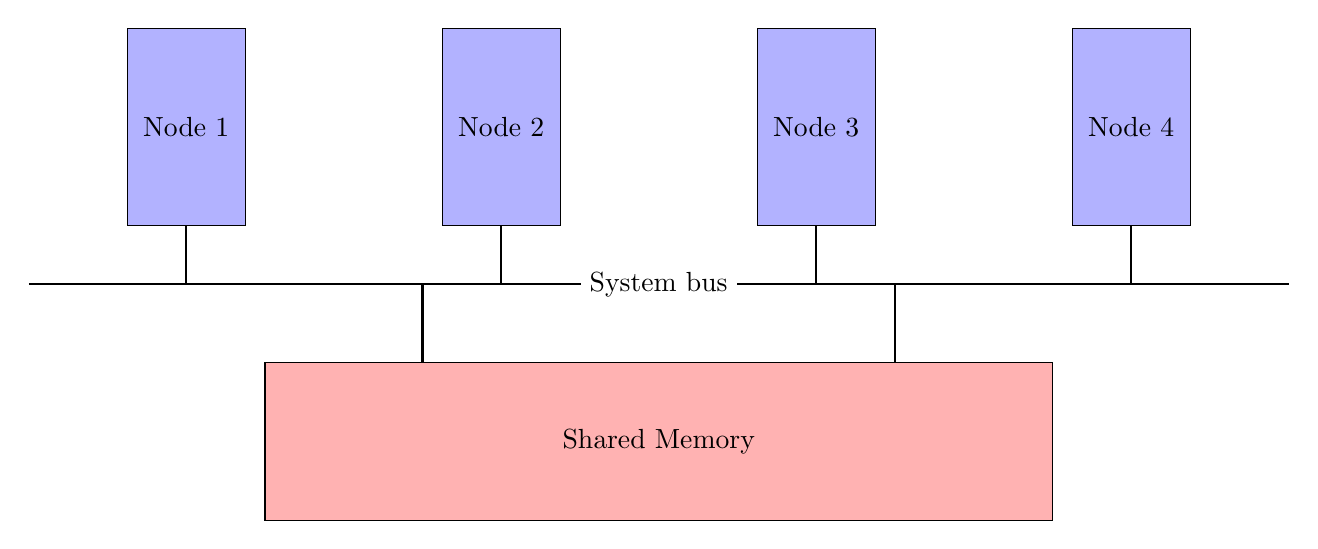
\begin{tikzpicture}
      % System \gls{bus}
      \draw[thick] (0,0) -- (16,0) node[pos=0.5, fill=white] {System bus};

      % Compute Nodes
      \foreach \x in {2, 6, 10, 14} {
          \node (CN\x) [draw, rectangle, minimum width=1.5cm, minimum height=2.5cm, fill=blue!30] at (\x, 2) {};
          \draw[thick] (\x,0) -- (CN\x);
        }

      % Labels for Compute Nodes
      \foreach \x [count=\xi] in {2, 6, 10, 14} {
          \node at (\x, 2) {Node \xi};
        }

      % Memory
      \node (MEM) [draw, rectangle, minimum width=10cm, minimum height=2cm, fill=red!30] at (8, -2) {Shared Memory};

      % Connections
      \foreach \x in {5,11} {
          \draw[thick] (\x,0) -- (\x,-1);
        }
    \end{tikzpicture}
  }
  \caption{Symmetric Multi-Processing (SMP) Architecture}
  \label{fig:smp}
\end{figure}

\ac{CPU} speed improvements outpacing memory technology led to the flat memory not being
able to keep up with the \ac{I/O} demand of the \ac{CPU}s; this problem has come to be commonly known as the \texttt{"von Neumann bottleneck"}.

\textbf{NUMA}

To alleviate this issue of the \texttt{"von Neumann bottleneck"} new, more distributed memory architectures have been developed.
The central idea is to create multiple smaller zones of collaboration  -- namely,
instead of having all cores having equal access to a single large chunk of memory,
allocating smaller chunks of memory to a few cores each which they can access quickly,
while still allowing them to access the memory of all other cores.
This prevents the issue of the \texttt{"von Neumann bottleneck"} by reducing the number of cores that need to access the same memory
while at the same time, but still allowing all cores to access the memory of all other cores.
This is what is called \ac{NUMA} architecture, as can be seen in Figure~\ref{fig:numa}.

\begin{figure}[!ht]
  \centering
  \vspace{0.5cm}
  \scalebox{0.9}{

    \begin{tikzpicture}

      % Nodes

      %node 1
      %CPU
      \node [draw, rectangle, minimum width=1cm, minimum height=1cm, fill=blue!30] (cpu11) at (-2, 2) {CPU1};
      \node [draw, below of=cpu11, rectangle, minimum width=1cm, minimum height=1cm, fill=blue!30] (cpu12) {CPU2};

      %Memory
      \node [draw, left=0.0cm of cpu11, rectangle, minimum width=2cm, minimum height=1cm, fill=red!30] (mem11) {Memory1};
      \node [draw, left=0.0cm of cpu12, rectangle, minimum width=2cm, minimum height=1cm, fill=red!30] (mem12) {Memory2};

      %Node box
      \node[draw,
        dashed,
        fit=(cpu11) (cpu12) (mem11) (mem12),
        inner sep=0.1cm,
        label={\scriptsize{Group 1}}
      ] (group1) {};

      %node 2

      %CPU
      \node [draw, rectangle, minimum width=1cm, minimum height=1cm, fill=blue!30] (cpu21) at (-2, -2) {CPU1};
      \node [draw, below of=cpu21, rectangle, minimum width=1cm, minimum height=1cm, fill=blue!30] (cpu22) {CPU2};

      %Memory
      \node [draw, left=0.0cm of cpu21, rectangle, minimum width=2cm, minimum height=1cm, fill=red!30] (mem21) {Memory1};
      \node [draw, left=0.0cm of cpu22, rectangle, minimum width=2cm, minimum height=1cm, fill=red!30] (mem22) {Memory2};

      %Node box
      \node[draw,
        dashed,
        fit=(cpu21) (cpu22) (mem21) (mem22),
        inner sep=0.1cm,
        label={\scriptsize{Group 2}}
      ] (group1) {};

      % node 3

      %CPU
      \node [draw, rectangle, minimum width=1cm, minimum height=1cm, fill=blue!30] (cpu31) at (2, 2) {CPU1};
      \node [draw, below of=cpu31, rectangle, minimum width=1cm, minimum height=1cm, fill=blue!30] (cpu32) {CPU2};

      %Memory
      \node [draw, right=0.0cm of cpu31, rectangle, minimum width=2cm, minimum height=1cm, fill=red!30] (mem31) {Memory1};
      \node [draw, right=0.0cm of cpu32, rectangle, minimum width=2cm, minimum height=1cm, fill=red!30] (mem32) {Memory2};

      %Node box
      \node[draw,
        dashed,
        fit=(cpu31) (cpu32) (mem31) (mem32),
        inner sep=0.1cm,
        label={\scriptsize{Group 3}}
      ] (group1) {};


      % node 4

      % CPU
      \node [draw, rectangle, minimum width=1cm, minimum height=1cm, fill=blue!30] (cpu41) at (2, -2) {CPU1};
      \node [draw, below of=cpu41, rectangle, minimum width=1cm, minimum height=1cm, fill=blue!30] (cpu42) {CPU2};

      %Memory

      \node [draw, right=0.0cm of cpu41, rectangle, minimum width=2cm, minimum height=1cm, fill=red!30] (mem41) {Memory1};
      \node [draw, right=0.0cm of cpu42, rectangle, minimum width=2cm, minimum height=1cm, fill=red!30] (mem42) {Memory2};

      %Node box
      \node[draw,
        dashed,
        fit=(cpu41) (cpu42) (mem41) (mem42),
        inner sep=0.1cm,
        label={\scriptsize{Group 4}}
      ] (group1) {};

      % interconnects

      \draw[thick] (cpu12) -- (cpu21);
      \draw[thick] (cpu11) -- (cpu31);
      \draw[thick] (cpu22) -- (cpu42);
      \draw[thick] (cpu32) -- (cpu41);

      \draw[thick] (cpu12) -- (cpu41);
      \draw[thick] (cpu32) -- (cpu21);


    \end{tikzpicture}
  }
  \caption{Three Tiered NUMA Architecture\protect\footnotemark}
  \label{fig:numa}
\end{figure}

\footnotetext{Diagram adapted from \cite{ploskasIntroduction2016}}

The diagram in \ref{fig:numa} shows a three-tiered \ac{NUMA} system, two processors having access to their own memory, while also being able to access the memory of the other processor.

\begin{enumerate}
  \item The \ac{CPU}s own cache which is the fastest to access.
  \item The cache of the \ac{CPU}s neighbor cores on the same group.
  \item The memory of the other groups.
\end{enumerate}

While this lets the \ac{SMP} systems scale much larger than the \ac{UMA} systems,
it also has to deal with the issue of keeping these distributed memory systems in sync,
as well as making sure to distribute this memory in a way that is optimal for the workload.


\textbf{Cache Coherence}

The problem of keeping the memory in sync is called \textit{cache coherence},
which is the process of making sure that every core has the same view of the memory\footcite{prof.dr.benh.juurlinkLectureCacheCoherence2018}.
If an operation on the memory is performed all other cores need to be informed about this change.
To do this efficiently, is a significant challenge, and many protocols have been developed to address this issue\footcite{hennessyComputerArchitectureQuantitative2011}.



% The former is called \textit{cache coherence} and is the process of making sure that every core has the same view of the memory.
% This is an issue because when a core modifies a piece of shared data, it takes a copy of that data in its own cache, and then writes back the data. 
% But if another core has also taken a copy of the same data, it will have an outdated version of the data, which could lead to inconsistencies 
% and race conditions. To prevent this, the cores need to coordinate with each other, to make sure that they have the same view of the memory\footcite{prof.dr.benh.juurlinkLectureCacheCoherence2018}.
% To address this issue several protocols have been conceived like the \ac{MESI} and \ac{MOESI} protocols, which is used in most modern systems\footcite{hennessyComputerArchitectureQuantitative2011}. 

% These protocols can be categorized into two main categories, the \textit{snooping} and the \textit{directory based} protocols.
% Snooping protocols are based on a shared \gls{bus}, where all cores can listen in on the communication between the core. 
% This is done either by updating the cache of all other cores directly or by sending a notification of invalidation\footcite{prof.dr.benh.juurlinkLectureClassesCache2018}.
% But as these are reliant on a shared \gls{bus}, they scale poorly with the number of cores, as the \gls{bus} becomes a bottleneck\footcite{prof.dr.benh.juurlinkLectureSMPLimitations2018}.

% As the \gls{bus} based communication is inherently limited in its scalability a more distributed approach was developed, the directory based protocols.
% So instead of broadcasting every change to all cores, we have a more direct form of communication like a point to point connection between the cores.
% Therefore only the cores that need to know about the change are informed, removing the strain on the interconnect as it now only needs to 
% facilitate the communication between those to cores\footcite{rajeevbalasubramonianLecture75Directory2015}. 
% But this system also needs to keep track of which core actually has a copy of the data, and which core needs to be informed about a change in the data.
% This is done via the directory, which stores a list of all sharing cores for each piece of data, and is responsible for keeping this list up to date.
% So whenever a core fetches data to its cache form another cores memory, the memory will log who requested the copy.
% And when a core writes back the data, the memory will only inform the cores that have a copy of the data, therefore reducing the overhead of the communication\footcite{prof.dr.benh.juurlinkLectureScalableCache2018}.

% % \TODO{Note from Harumi: I think you must be doing fine with regard to content, but if you need more, you could write something here about false sharing.}
% %  Yes I even started writing a section about it because I found an excellent OpenMP talk about the issues with this.
% % I found it: https://www.youtube.com/watch?v=u6N33FhfgZU

\textbf{Memory Placement}
\label{sec:memory_placement}

A second issue is how to distribute memory across different nodes in such a way that the overall access time is minimized.
As memory is spread across many nodes, which are of different accessibility, it becomes especially important where the memory is initially placed.
and how it is spread across the nodes. The default behavior of \textit{OpenMP} is to place the whole data on the first node that accesses it,
which is called \textit{first touch} policy. This is done to reduce the overhead of the communication, as the data is already on the node that needs it.
But even in the very baseline case, where more than one core needs to access the same data, the data will be entirely placed on the first node that accesses it,
needing to manually instructed to distribute the ownership of the data across the nodes\footcite{ruudvanderpasSpeedYourOpenMP}.



% - promlems with numa
%   - false sharing
%      - changing shared cache lines often results in lots of overhead through cache coherence protocols
%      - recomendet to use private data first if you want to edit a lot


\textbf{Distributed Memory}

While memory sharing systems have come a long way in scaling and performance and have a strong foothold in multi-core systems,
they are still limited in their scalability and flexibility, as they are limited to a single system both physically and by operating system\footcite{hpcwikiParallelProgramming}.
The solution to this are distributed memory systems which take the opposite approach to the shared memory systems; instead of having the entire memory available to all cores all
working on the same problem, the memory is instead private to each core. Therefore instead of having a single large memory, be it uniform or not the memory is split into separate chunks.
This is especially useful for problems that are not tightly coupled, as the cores can work on their own data without the need to communicate with the other cores.
The way the cores communicate is by passing messages over the network, which is much slower than the shared memory communication, but also much more scalable, how this
is done specifically is discussed in the section \ref{sec:message_passing}.
A welcome side effect of this is its compatibility with commodity hardware, as the nodes do not need the physical ability to support shared memory,
enabling the use of off the shelf hardware, which was a significant factor in the rise of \ac{HPC} clusters and \ac{CC} systems\footcite{dongarraHighperformanceComputingClusters2005}.



\textbf{Hybrid Systems}

Similar to how the \ac{NUMA} systems are a more distributed version of the \ac{UMA} systems having smaller zones of fast access,
modern \ac{HPC} systems take on a hybrid approach.
The current trend in \ac{HPC} is to combine the best of both worlds, utilizing many commodity multi-core \ac{NUMA} nodes,
combined via a high-speed network, to form a distributed memory system \footcite{rabenseifnerHybridMPIOpenMP2009}
While most of these systems are either based on extensions of the \ac{MPI} standard in order to support
local shared memory communication, alternative approaches have been developed to support this hybrid approach
on a more fundamental level \footcite{jinHighPerformanceComputing2011}.

One such approach is the \ac{PGAS} model, which try to utilize the best of both worlds by letting the programmer
control the memory placement, while still having the ability to communicate between the nodes.
The way this is done is create the perception of a single large memory, while in reality the memory is distributed across the nodes,
and in order to describe the topology of the address space, as it is not uniform in accessability, the memory is partitioned into segments\footcite{dewaelPartitionedGlobalAddress2015}.
The distance or the cost of using a remote memory access is then modeled by the specific implementing library,
which either optimizes the placement and access of the memory implicitly, or lets the developer explicitly control the placement of the memory\footcite{almasiPGASPartitionedGlobal2011}.
One of the distinguishing factors of \ac{PGAS} is the one sided communication, as foreign memory can be directly
accessed via \ac{RDMA} operations without needing to involve the other core\footcite{dewanPavingWayDistributed2020}.


% hybrid infrastructure,
% extremly common
% multiple nodes are interconnected via a network connection, while each node has multiple cores, which can access a shared memory, but also have their own cache.

\subsubsection{Networking and Interconnects}
\label{sec:networking_interconnects}

As the communication between the nodes is one of the most significant bottlenecks in \ac{HPC} systems, the interconnects are a crucial part of the system.
The two significant factors when it comes to interconnects is the kind of network fabric used as well as the topology of the network itself\footcite{bestaHighPerformanceRoutingMultipathing2021}
On the chip level the communication is done via the process interconnects which communicate between the cores and memory, while on the cluster level the
communication is done via a network fabric, interconnecting the nodes through a high speed network connection\footcite{dongarraHighperformanceComputingClusters2005}.

When talking about the network fabric, the most common types of network fabrics used in \ac{HPC} are Ethernet and InfiniBand,
each having roughly 40\% of the market share, with no significant difference even when weighed by performance\footcite{top500ListStatisticsInterconnect}.


Ethernet has been the default network connection for most devices for decades, resulting in a high availability of hardware and software support,
while being highly flexible and relatively cheap. But as it was designed for general purpose \ac{LAN} and \ac{WAN} communication,
it, in its standard form not originally designed for high speed communication between nodes\footcite{howardInfiniBandVsEthernet2023}.
The largest issue with baseline Ethernet is that it does not natively support \ac{RDMA} operations which is a very specific
requirement for \ac{HPC} systems, as it enables the direct access of memory between the nodes, without the need to involve the \ac{CPU}\footcite{rdmaconsortiumRDMAConsortiumFAQs2003}
To solve this issue the \ac{iWARP} protocol was developed, enabling to use the entire Ethernet stack for the infrastructure,
while letting special \ac{RDMA} capable \ac{NIC}s handle the communication\footcite{intelUnderstandingIWARPDelivering2010}.
But \ac{iWARP}, being dependent on the \ac{TCP/IP} stack is not as fast as the native \ac{RDMA} capable InfiniBand,
which is a specialized network fabric designed for high speed communication between nodes.
In order to close this gap between the two, the \ac{RoCE} protocol was developed, providing better performance and
lower latency than \ac{iWARP}, while still being able to use the existing Ethernet infrastructure while being on par with InfiniBand\footcite{howardInfiniBandVsEthernet2023}.

In contrast to Ethernet, InfiniBand was designed from the ground up for high speed communication between nodes in a cluster.
It is a very low latency, high bandwidth network fabric, which native supports \ac{RDMA} operations, but requires specialized hardware and software support
as well as being a proprietary standard, which can lead to higher costs and less flexibility\footcite{pfisterIntroductionInfiniBandArchitecture}.

The choice of network fabric is highly dependent on the specific use case, as Ethernet is more flexible and cheaper, while InfiniBand is faster and more specialized.
But as can be seen in the \ac{HPC} Top500 list, both are relatively equally represented in the top systems, showing that both are viable options\footcite{top500ListStatisticsInterconnect}.

\textbf{Network Topology}
\label{sec:network_topology}

No matter which network fabric is used, the topology of the network is also a significant factor in the performance of the system, as the topology
becomes more expensive and complex as the number of nodes increases. The topology of the network is the way the nodes are connected to each other,
essentially being the structure of the whole supercomputer.

Below are three very simplified examples of network topologies which each demonstrate the central problems of network topologies, between which the system architect has to balance:
One needs to keep in mind, that while these only have 8 nodes each the actual systems can have thousands of nodes which need to be connected.
The three most important factors when it comes to network topologies are the diameter, the bisection bandwidth as well as the cost of the network\footcite{bestaHighPerformanceRoutingMultipathing2021b}.

First, the \textit{Star Topology} in figure \ref{fig:star_top} shows that all nodes are connected to a central switch.
This configuration ensures that each node can directly communicate with every other node with a single hop, resulting in a low diameter connection.
But as the entire communication has to go through the central switch, the entire communication has to go through the central switch, the bisection bandwidth is ultimately limited by the capacity of this central hub.
This presents a scalability issue; as the number of nodes increases, the central switch becomes a potential bottleneck, impacting the overall system performance. Moreover, the cost and complexity associated with upgrading or maintaining such a central switch can be prohibitively high for larger networks.

\begin{figure}[!ht]
  \centering
  % Start of the first minipage for the star topology
  \begin{minipage}{0.3\textwidth}
    \centering
    \scalebox{0.6}{
      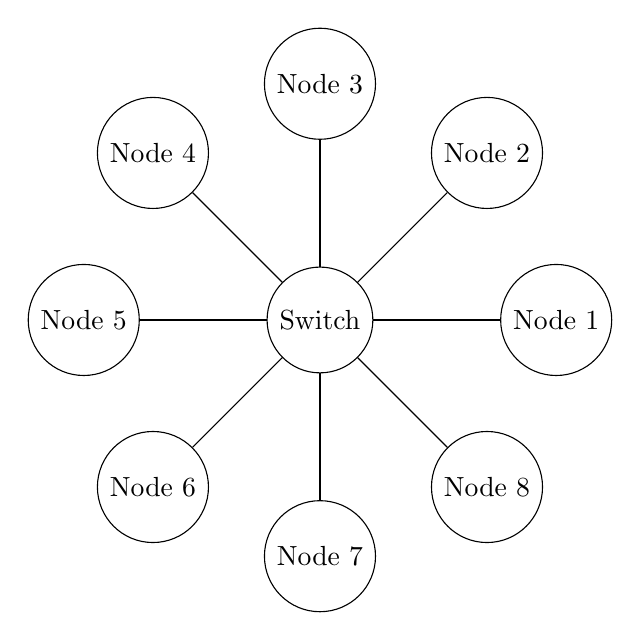
\begin{tikzpicture}
        % Number of nodes
        \def\numNodes{8}
        % Central node
        \node[draw, circle] (central) at (0,0) {Switch};

        % Calculate angle step based on the number of nodes
        \pgfmathsetmacro{\angleStep}{360/\numNodes}

        % Generate nodes in a circle
        \foreach \n in {1,...,\numNodes}{
            % Calculate angle for this node
            \pgfmathsetmacro{\angle}{\angleStep*(\n-1)}

            % Position node using polar coordinates
            \node[draw, circle] (Node\n) at (\angle:3cm) {Node \n};
          }

        % Draw connections between all nodes
        \foreach \i in {1,...,\numNodes}{
            \draw (Node\i) -- (central);
          }
      \end{tikzpicture}
    }
    \caption{Star Topology}
    \label{fig:star_top}
  \end{minipage}
  \hfill % Use \hfill to push the minipages to their respective sides
  % Start of the second minipage for the ring topology
  \begin{minipage}{0.3\textwidth}
    \centering
    \scalebox{0.6}{
      \begin{tikzpicture}
        % Number of nodes
        \def\numNodes{8}
        % Calculate angle step based on the number of nodes
        \pgfmathsetmacro{\angleStep}{360/\numNodes}

        % Generate nodes in a circle
        \foreach \n in {1,...,\numNodes}{
            % Calculate angle for this node
            \pgfmathsetmacro{\angle}{\angleStep*(\n-1)}

            % Position node using polar coordinates
            \node[draw, circle] (Node\n) at (\angle:3cm) {Node \n};

            % Connect each node to the next, creating a ring
            \pgfmathtruncatemacro{\nextNode}{mod(\n,\numNodes)+1}
            \draw (Node\n) -- (Node\nextNode);
          }
      \end{tikzpicture}
    }
    \caption{Ring Topology}
    \label{fig:ring}
  \end{minipage}
  \hfill % Use \hfill again for spacing
  % Start of the third minipage for the fully connected graph
  \begin{minipage}{0.3\textwidth}
    \centering
    \scalebox{0.6}{
      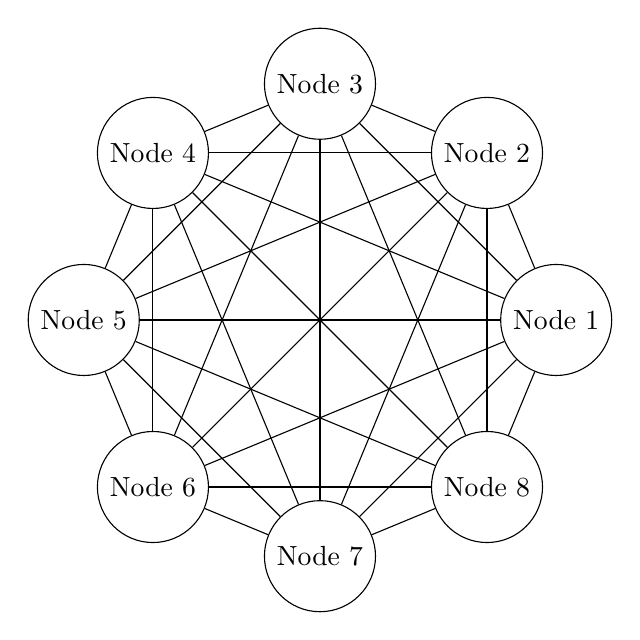
\begin{tikzpicture}
        % Number of nodes
        \def\numNodes{8}

        % Calculate angle step based on the number of nodes
        \pgfmathsetmacro{\angleStep}{360/\numNodes}

        % Generate nodes in a circle
        \foreach \n in {1,...,\numNodes}{
            % Calculate angle for this node
            \pgfmathsetmacro{\angle}{\angleStep*(\n-1)}

            % Position node using polar coordinates
            \node[draw, circle] (Node\n) at (\angle:3cm) {Node \n};
          }

        % Draw connections between all nodes
        \foreach \i in {1,...,\numNodes}{
            \foreach \j in {\i,...,\numNodes}{
                \ifnum\i=\j\relax
                  % Skip drawing a node to itself
                \else
                  \draw (Node\i) -- (Node\j);
                \fi
              }
          }
      \end{tikzpicture}
    }
    \caption{Connected Graph}
    \label{fig:fully_connected}
  \end{minipage}
  % End of the third minipage
\end{figure}


Next, the \textit{Ring Topology} depicted in figure \ref{fig:ring} is examined, where each node is connected to two other nodes,
forming a loop. This topology allows for a straightforward path of communication, with data traveling around the ring to reach its destination.
The diameter of this topology grows linearly with the number of nodes, making it less ideal as the network size increases.
% \todo{Note from Harumi: I swapped the following two sentences because I thought it read better that way given that the previous sentence gives a negative.}
On the plus side, the ring topology is relatively inexpensive to implement and scale, as adding more nodes simply involves creating two additional connections for each new node.
However, the bisection bandwidth of a ring topology is inherently limited, cutting the ring at any point to form two halves only requires severing two connections,
which could easily become a bottleneck in data-intensive applications.

Finally, the \textit{Fully Connected Network}, as shown in figure \ref{fig:fully_connected}, offers the most direct communication paths, with each node directly connected to every other node.
This topology boasts the lowest possible diameter of 1, as any two nodes can communicate directly without intermediary nodes.
The bisection bandwidth in this topology is maximized, given the sheer number of connections that would need to be severed to bisect the network.
However, the cost and complexity associated with a fully connected network are its most significant drawbacks.
The number of required connections grows quadratically with the addition of nodes, making this topology impractical for large-scale applications due to the prohibitive cost of implementing and maintaining such an extensive network.

In practice, most \ac{HPC} systems utilize a combination of these topologies, such as the \nameref{fig:fat_tree} (\ref{fig:fat_tree}) or \nameref{fig:hypercube}(\ref{fig:hypercube}), which strike a balance between performance, scalability, and cost\footcite{bestaHighPerformanceRoutingMultipathing2021b}.


\begin{figure}[!ht]

  \centering
  \vspace{0.5cm}
  \begin{minipage}{0.5\textwidth}
    \centering
    \scalebox{0.5}{
      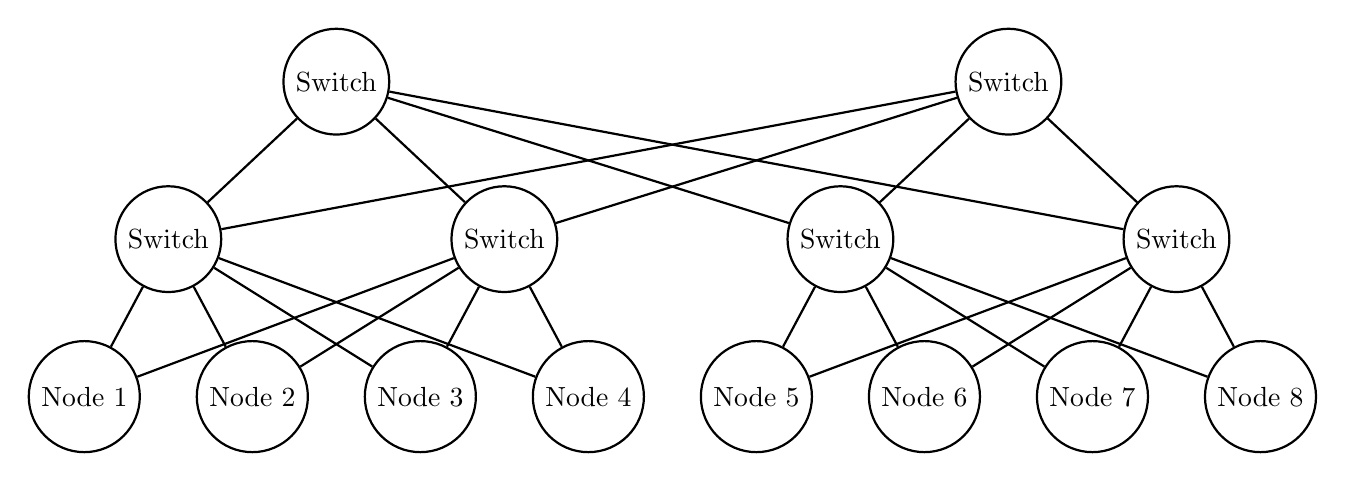
\begin{tikzpicture}[node distance={15mm}, thick, main/.style = {draw, circle}]
        \def\numNodes{8}
        \def\levelSep{2cm}
        \def\nodeSep{0.75mm}

        % Drawing the root switches 
        \pgfmathsetmacro{\nodesInRoot}{\numNodes/4}
        \foreach \i in {1,...,\nodesInRoot}{
            \pgfmathsetmacro{\xPos}{(\i - (\nodesInRoot+1)/2)*(4*\nodeSep)}
            \node[draw, circle] (root-\i) at (\xPos, 0) {Switch};
          }

        % Drawing the first level of switches
        \pgfmathsetmacro{\nodesInLevel}{\numNodes/2}
        \foreach \i in {1,...,\nodesInLevel}{
            \pgfmathsetmacro{\xPos}{(\i - (\nodesInLevel+1)/2)*(2*\nodeSep)}
            \node[draw, circle] (level1-\i) at (\xPos, -\levelSep) {Switch};
          }

        % Drawing the base nodes
        \foreach \i in {1,...,\numNodes}{
            \pgfmathsetmacro{\xPos}{(\i - (\numNodes+1)/2)*\nodeSep}
            \node[draw, circle] (base-\i) at (\xPos, -2*\levelSep) {Node \i};
          }

        % Connections
        % Root routers to each layer 1 router
        \foreach \root in {1,...,\nodesInRoot}{
            \foreach \lvlOne in {1,...,\nodesInLevel}{
                \draw (root-\root) -- (level1-\lvlOne);
              }
          }

        % Layer1 router 1 and 2 to nodes 1-4
        \foreach \i in {1,...,4}{
            \draw (level1-1) -- (base-\i);
            \draw (level1-2) -- (base-\i);
          }

        % Layer1 router 3 and 4 to nodes 4-8
        \foreach \i in {5,...,8}{
            \draw (level1-3) -- (base-\i);
            \draw (level1-4) -- (base-\i);
          }
      \end{tikzpicture}
    }
    \caption{Fat Tree Topology}
    \label{fig:fat_tree}
  \end{minipage}\hfill
  \begin{minipage}{0.5\textwidth}
    \centering
    \scalebox{0.5}{
      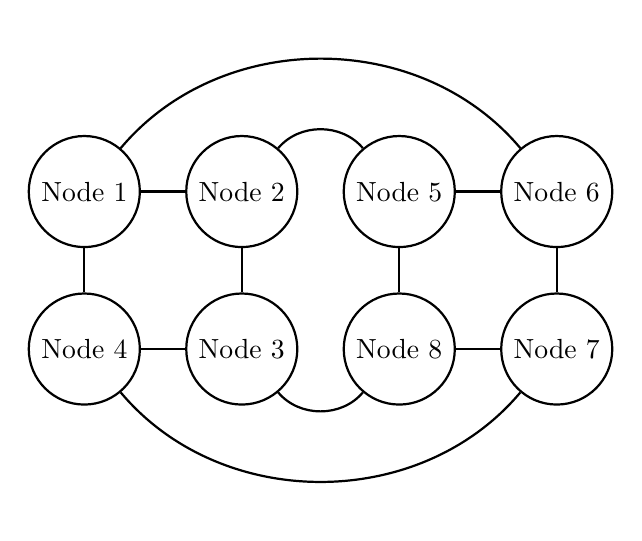
\begin{tikzpicture}[node distance={2cm}, thick, main/.style = {draw, circle}]
        % Nodes
        \node[main] (1)              {Node 1};
        \node[main] (2) [right of=1] {Node 2};
        \node[main] (3) [below of=2] {Node 3};
        \node[main] (4) [below of=1] {Node 4};
        \node[main] (5) [right of=2] {Node 5};
        \node[main] (6) [right of=5] {Node 6};
        \node[main] (7) [below of=6] {Node 7};
        \node[main] (8) [below of=5] {Node 8};

        % Connections
        \draw (1) -- (2);
        \draw (1) -- (4);
        \draw (2) -- (3);
        \draw (3) -- (4);
        \draw (1) edge[bend  left=50] (6); % Arching connection
        \draw (2) edge[bend  left=50] (5); % Arching connection
        \draw (3) edge[bend right=50] (8); % Arching connection
        \draw (4) edge[bend right=50] (7); % Arching connection
        \draw (5) -- (6);
        \draw (6) -- (7);
        \draw (7) -- (8);
        \draw (8) -- (5);
      \end{tikzpicture}
    }
    \caption{Hypercube Topology}
    \label{fig:hypercube}
  \end{minipage}
\end{figure}

% % \todo{should I use routing or switching? as IB uses switching and TCPIPoEthernet uses routing.  Note from Harumi: https://www.baeldung.com/cs/routing-vs-forwarding-vs-switching Routing is moving data between nodes; Switching is a subset of routing -- moving data from a node to multiple nodes. Are you asking about the figure? I think switch is correct there.}

% While there exist many more complex topologies, like \texttt{Dragonfly} or \texttt{Torus} topologies they 
% all trade off between the diameter, the bisection bandwidth and the cost according to the specific use case.


% % \footcite{eickhoffTopologyAwareWorkloadAnalyzer} also explains low diameter and high diversiyu topologies are important for HPC systems.
% % Explain the concepts of network topology and how different topologies (e.g., fat tree, torus, hypercube) impact performance.


% % % Storage Systems

% %     Elaborate on hierarchical storage management and the role of parallel file systems (e.g., GPFS, Lustre) in HPC.
% %     Address the challenges of I/O bottlenecks and how they can be mitigated.

\subsection{HPC Software Stack}

Now that we have discussed the hardware components and their configurations, we will dive into the software stack that powers \ac{HPC} systems.
While this is the only part we can directly interact with as developers, many of the decision made in the hardware stack have a direct impact on
the software we will be working with on the cluster.


\subsubsection{Operating Systems}
\label{sec:operating_systems}

% \todo{Note from Harumi: I heavily edited the following paragraph.}
% Haha Linux history is propably the most controversial part of the whole paper. :D
While the operating system is the most fundamental part of modern computers, in the context of \ac{HPC} systems there exists no competition to the Linux operating system,
which has had a 100\% market share in the \ac{HPC} Top500 list since 2017\footcite{top500OperatinststemsDevelopmentTime}.
Before its rise to dominance, Linux's competitors were its predecessors -- other, proprietary, UNIX-based operating systems that were
the default operating systems for most \ac{HPC} systems.
%But the \ac{HPC} community is complexly directed towards \gls{POSIX}-compliant systems\footcite{top500OperatinststemsDevelopmentTime}.
Linux has come to dominate the \ac{HPC} community for a number of reasons that include a desire to avoid vendor lock-in and licensing costs,
as well as an appreciation for the customizability and flexibility of Linux,
as its Kernel, Software and Libraries are all open source, which enables the community to optimize the system for their specific use case\footcite{rohitguptaLinuxOperatingSystem}.


\subsubsection{Programming Models}
\label{sec:programming_models}
As already mentioned above, the way the hardware works in \ac{HPC} systems is very closely tied into the way the software needs to be written.
This is especially true for this section, as the way the memory is distributed across the nodes and how the cores communicate with each other
,needs to be taken into account when writing the software, or at least assumed by the framework that is used.


\textbf{OpenMP}

OpenMP is a shared memory parallel programming model, it is the software counterpart of the \ac{SMP} hardware architecture, and works both with \ac{UMA} and \ac{NUMA} systems.
It is a set of compiler directives, library routines, and environment variables that enable the parallelization of code on shared memory systems \footcite{hermannsParallelProgrammingFortran}.
So it is designed to work on a single node of a given cluster, but able to utilize and combine the power ot the cores and memory of the whole node,
but cannot go beyond the boundaries of the node and communicate with other nodes\footcite{mitplasmascienceandfusioncenterIntroParallelProgramming2022}.
Compared to other parallel programming models, OpenMP presents a relatively high level of abstraction, being able to parallelize code with a few lines of code.
Its main advantage is its simplicity. OpenMP is based on compiler directives, which are added to the code and interpreted by the compiler to generate the parallelized code.
This makes it very easy to use, as the programmer does not need to worry about the specifics of the hardware as the compiler will take care of it\footcite{niklaswittmerParallelisierungMitOpenMP2018}.
While this is a great advantage for the programmer and lowers the barrier of entry for subject-matter experts of a specific field, it also has its drawbacks.
As the compiler makes relatively uninformed decisions about the parallelization, the performance of the parallelized code can be suboptimal\footcite{ruudvanderpasGettingOpenMPSpeed2014}.

It implements parallelization using a multithreaded fork-join model, where a single thread starts the program and then forks additional threads to run the parallelized code as can be seen in figure \ref{fig:fork_join} below.
So once a parallel region is defined by the programmer the process will fork the specified number of threads, which will run concurrently until the end of the region, where they join back together to continue the sequential execution of the code\footcite{laboratoryOpenMPProgrammingModel}.
While these threads are running concurrently, they have access to a shared memory space containing the previous linear state of the program,
but also have their own private memory space, which is used to store the variables that are only relevant to the specific thread\footcite{mitplasmascienceandfusioncenterIntroParallelProgramming2022}.

\begin{figure}[!ht]
  \centering
  \scalebox{0.8}{
    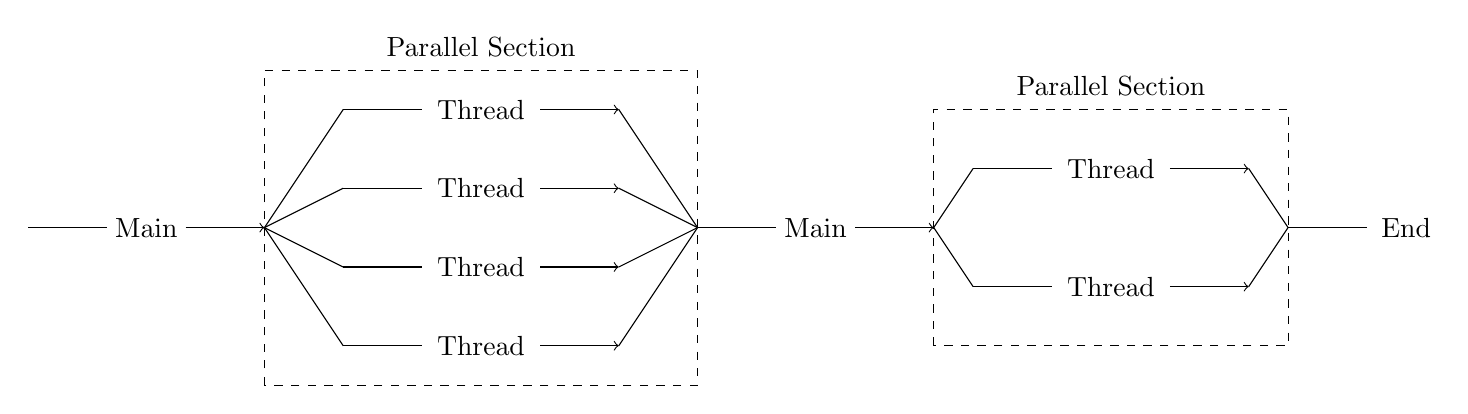
\begin{tikzpicture}[node distance=0.5cm and 1cm]
      % Main thread
      \draw (0,0) -- (1,0);
      \node at (1.5,0) {Main};
      \draw[->] (2,0) -- (3,0);
      % Linear Section Label

      % First Parallel Section Box
      \draw [black, dashed] (3,-2) rectangle (8.5,2);
      \node at (5.75,2.3) {Parallel Section};

      % Fork 1 x4 
      \foreach \y in {1.5, 0.5, -0.5, -1.5}{
          \draw (4,\y) -- (5,\y);
          % drawing connection to main 
          \draw (3,0) -- (4,\y);
          \node at (5.75,\y) {Thread};

          \draw[->] (6.5,\y) -- (7.5,\y);
          \draw (7.5,\y) -- (8.5,0);
        }

      \draw(8.5,0) -- (9.5,0);
      \node at (10,0) {Main};
      \draw[->] (10.5,0) -- (11.5,0);

      % Second Parallel Section Box
      \draw [black, dashed] (11.5,-1.5) rectangle (16,1.5);
      \node at (13.75,1.8) {Parallel Section};

      % fork 2 x2
      \foreach \y in {0.75, -0.75}{
          \draw (12,\y) -- (13,\y);
          % drawing connection to main 
          \draw (11.5,0) -- (12,\y);
          \node at (13.75,\y) {Thread};

          \draw[->] (14.5,\y) -- (15.5,\y);
          \draw (15.5,\y) -- (16,0);
        }

      \draw(16,0) -- (17,0);
      % draw end 
      \node at (17.5,0) {End};
      % Join Label

    \end{tikzpicture}
  }
  \caption{Fork-Join Model}
  \label{fig:fork_join}
\end{figure}
For example, a loop that would normally be executed sequentially can be parallelized with OpenMP
by adding the \texttt{\#pragma omp parallel for} directive in front of the loop.
This will tell the compiler to parallelize the loop, and the compiler will then generate the code to run the loop in parallel\footcite{mitplasmascienceandfusioncenterIntroParallelProgramming2022}.
On runtime instead of going through each iteration of the loop one by one,
all the iterations will be divided between the threads, which will then run the iterations concurrently.
The program then waits for all threads to finish before continuing.


\textbf{Message Passing}
\label{sec:message_passing}

If OpenMP is the standard for shared memory systems, then the \ac{MPI} is its equivalent for distributed memory systems.
It is a standardized and portable message-passing system designed to work on a wide variety of computers, and is language independent, supporting C, C++, and Fortran\footcite{groppUsingMPIPortable1999}.
In practical terms, \ac{MPI} serves as an \ac{API} that enables the inter-process communication across nodes and the network,
allowing the programmer to send and receive messages between the nodes, and to synchronize the processes\footcite{vishuvaishnavMessagePassingDistributed2023}.

While some implementations enable the use of shared memory within a node, which have become a valuable tool in hybrid systems,
\ac{MPI} itself is primarily designed around the actively sending and receiving messages
during runtime instead of accessing the memory directly.

\ac{MPI} is based on the \ac{SPMD} model, where each process runs the same program, but with different data, and can communicate with each other via messages.
This is done via the so-called \textit{rank} of the process, which is a unique \ac{ID} assigned to each process,
serving as an address for the process, used to send and receive the messages, without needing
to concern itself with the specifics of the underlying \gls{ISO/OSI model}\footcite{openmpiWhatOpenMPI2014}.

Messages in \ac{MPI} are sent and received either via point-to-point communication where the \textit{rank} of the sender and receiver are specified,
or via a collective communication, where information is sent or received from all or a subset of the processes\footcite{eickhoffTopologyAwareWorkloadAnalyzer}.
These collective operations can be split into two dimensions:

\begin{enumerate}
  \item \textbf{Data flow direction:} As a process can either send or request the reception of a message, the flow of communication can be either towards
        the initiating process, so a process might send a subtask to other processes(e.g. \textit{BROADCAST}) or request the results of a subtasks in order to continue(eg. \textit{GATHER})\footcite{dartmouthcollegeMPICollectiveCommunication}.
  \item \textbf{Data distribution:}
        The data a process sends/receives can either be a single value being replicated  across all processes (e.g. \textit{BROADCAST}) or a number of values being spread across the processes (eg. \textit{SCATTER})\footcite{dartmouthcollegeMPICollectiveCommunication}.
\end{enumerate}

% \todo{Maybe here I should add diagramm witht the different collective operations as matrixes like in the citation}

% The second important feature of \ac{MPI} is how and whether communication completeness is checked.
% As the default behavior of \ac{MPI} is to block until the message is send/received, the communication is inherently synchronous.
% This can leave some performance on the table, as the communication between the nodes is quite slow compared to the communication between the cores,
% therefore \ac{MPI} also provides non-blocking functions, which will return immediately, and the program can continue to run while the message is being send or received\footcite{shunyancheungAsynchronousCommunicationPrimitives}.

\textbf{Chapel/GASNet}
\label{sec:gasnet}

If OpenMP is the standard for shared memory systems, and \ac{MPI} is the standard for distributed memory systems, then Chapel is the standard for \ac{PGAS} systems.
Chapel is a high-level parallel programming language designed for productive parallel computing across a wide range of scales, from multi-core desktops to the supercomputers\footcite{chapel-lang.orgChapelOverview}.
Being based on the \ac{GASNet}, Chapel is able to work on both shared, distributed memory systems and hybrid systems, or even emulating multiple nodes on a \ac{SMP} system for development and testing\footcite{chapel-lang.orgMultilocaleChapelExecution}.
Making use of \ac{RDMA} in order to present a part of the memory as a large combined memory space, while in reality the memory is distributed across the nodes.
Being able to directly accessing the memory across the network, avoiding the overhead of the \ac{CPU} and the \ac{OS} in order to send and receive messages,
also has the advantage of being inherently asynchronous, as the memory can be directly accessed without needing to wait for the other process to be ready\footcite{dewanPavingWayDistributed2020}.

While some \ac{MPI} implementations such as \texttt{MVAPICH} or \texttt{OpenMPI} have started to implement \ac{RDMA} capabilities,
and \ac{GASNet} also supports network stacks which are not directly \ac{RDMA} capable,
each of these implementations was written with a specific use case in mind are oriented towards a specific use case.
An example for this is \ac{GASNet}s ability to access memory directly is not just limited to the \ac{CPU} memory,
but can also directly connect to auxiliary compute devices such as \ac{GPU}s in order to offload the
computations to the corresponding coprocessor\footcite{chamberlainPROGRAMMINGLANGUAGEPRODUCTIVE}.

\subsubsection{Workload Management Systems}

% \todo{Note from Harumi: are you allowed to write in the first person? I personally write "we" all the time, but I think this is the first time you have used it in this thesis.}
% So now that we have discussed how the hardware works on the nodes,
% Correction:
With an understanding of how the hardware works on the nodes,
how the cores can communicate with each other, even across the network,
and how these networks can be structured, the next step is to discuss
how when and where the code is being executed on the cluster.
This is where the workload management systems come into play, also known as schedulers or Batch systems,
as most of these systems main feature is the scheduler and primarily rely on a batch based distribution of jobs\footcite{hovestadtSchedulingHPCResource2003}.

The workload manager distributed jobs across the compute cluster.
Working with a list of computation tasks which are submitted by the users along with the
amount of resources they need, the workload manager is responsible for the distribution of the jobs across the cluster.
In order to optimize the utility of the cluster, the workload manager reduces the idle time of the nodes,
by fitting in as many jobs of different users as possible, trading off between quick execution and fairness\footcite{hpcwikiSchedulersHowToRunApplicationsonasupercomputer}.

One of the most common workload management systems is \ac{SLURM}, which is an open-source workload manager targeted towards \ac{HPC} systems\footcite{yooSLURMSimpleLinux2003}.
From the perspective of the user, \ac{SLURM} is a command line tool, which is used to submit jobs to the cluster
and from the perspective of the node it is a simple \gls{daemon} not to different from a remote shell\footcite{schedmdSlurmWorkloadManagera}.
But under the hood it is a highly complex system, checking the availability of the resources,
managing permissions and most importantly deciding the order of the jobs to be executed.
In its most basic form \ac{SLURM} is a \ac{FIFO} queue, where the jobs are executed in the order they are submitted,
which would lead to a low utilization of the cluster. Therefore, it does not strictly adhere to the \ac{FIFO} principle,
but slots in a lower priority job if it is able to run in a slot between regularly scheduled ones, as log as it does not delay any job of higher priority\footcite{schedmdSlurmWorkloadManagerb}

Additionally, \ac{SLURM} can be provided with information about the topology of the network,
supporting both torus and fat tree topologies, which can be used to optimize the placement of the jobs on the cluster,
by using an n-dimensional space filling curve in the former and a tree based algorithm in the latter in order to get the jobs
as close to each other as possible\footcite{schedmdSlurmWorkloadManagerc}.

\pagebreak

% Conceptual Deductive Analysis about Exploratory Computing
\section{Exploratory Computing}
\label{sec:EC}

With the advent of Big Data, the increasing complexity and increase of easily available 
compute resources, the field of data analysis has been under an ever-increasing pressure 
to "make sense" of the abundant data.
This need has given rise to the methodology of \acf{EC}, which is an iterative 
process of data analysis which maintains a close to real-time dialogue between the
analyst and the data\footcite{diblasExploratoryComputingDraft2014}.

Unlike conventional data analysis methods which might follow a straighter path towards
an answer to a specific question, \ac{EC} aims to be a more open-ended process, where the eventual goal is
not just to find a numerical answer to a question but rather to gain a deeper understanding of the dataset.
Therefore, the tools in this field require a high degree of interactivity in order to
become a more natural extension of the analysts thought process\footcite{grangerJupyterThinkingStorytelling2021}.

\textbf{Computational Notebooks}

The defacto standard for scientific \ac{EC} is the \textit{Computational Notebook},
allowing for the direct integration of narrative text, code, and it's output like visualizations, tables and other data structures.
While in some domains other notebooks systems like \textit{Wolfram Mathematica} and \textit{Matlab} are used,
the most common notebook especially in the field of data science is the \textit{Jupyter Notebook}\footcite{perkelWhyJupyterData2018}.

\textit{Jupyter Notebooks} is a \ac{FOSS} server-(web)client application that exposes 
an interactive editor.
User can write code, documentation and visualizations into so-called cells. 
These cells are then executed on the server, which can be local or a remote compute resource,
and the output is displayed in the notebook.
As the computational environment is preserved across cells, 
with each cell being able to access the variables and functions defined in previous cells.
This lends itself to the \ac{REPL} style of programming, without the need to re-run the whole script\footcite{jupyter-docsProjectJupyterDocumentation}.
One of the key features of \textit{Jupyter Notebooks} is the ability to run code in multiple languages,
as the server on the  backend is build on a modular architecture that allows for the integration of \textit{kernels}.
These kernels are responsible for executing the code in the cells and returning the output to the notebook,
but are only limited by the \ac{API} spec of the notebook server\footcite{jupyter-docsArchitectureJupyterDocumentation}.
This has lead to a wide variety of kernels being available, with the most common ones being for \textit{Python}, \textit{R} and \textit{Julia},
but also supporting languages which are not traditionally associated with data analysis like \textit{Postsript}, \textit{PowerShell} and \textit{Brainfuck}\footcite{jupyter-docsJupyterKernels}. 

\pagebreak

% Combined Conceptual Deductive Analysis
% \section{Combined Conceptual Deductive Analysis}
\section{Deductive Design of Conceptual Architecture}

Based on the deep knowledge gained by the previous sections,
it is now possible to create a combined conceptual approach to address the issues
described in the \nameref{Introduction} and the \nameref{ProblemStatement} sections.
This approach will be used as a guideline for the prototype implementation int the chapter \nameref{ArtifactDevelopment}.

In contrast to the sections above which went from the basic principles towards the higher levels of abstraction,
this chapter will start at the high level goals, their implications and what will be needed on the lower levels
in order to accomplish these goals.

\subsection{Goals}
\label{sec:goals}

Based on the \nameref{ProblemStatement}, the goals of the system can be summarized as follows:

% Original problem statement:
% While low latency high performance computing has been a focus of the HPC as well as the
% CC community, resulting in systems such as JupyterHub or Dask, these systems are inherently
% ephemeral and do not provide a way to reproduce results on a HPC scale. Therefore we need to
% solve the following problems:
% • P1: The GitOps first approach with introduces a latency between the changes made and
% the deployment of the new workflow. This latency prevents a real-time exploitive workflow
% and limits the usability for the interactive exploration of the data.
% • P2: Existing solutions for interactive workloads are inherently ephemeral and do not pro-
% vide a way to reproduce the results on a HPC scale


The designed system should provide the user with an easy-to-use interface,
capable of interactively exploring \ac{HPC} scale data.
The system should be able to run on cloud infrastructure, be able
to allocate the necessary resources, as well as scheduling and executing
the computation within a reasonable time frame.

% Yeah honestly it was not realistic to expect that I would be able to build a system which 
% could run HPC on the cloud just like that, while also seamlessly autoscaling and being cheap lol
% considering that this needed to be done within two months while writing this thesis at the same time.
% I got so close tho :(

% Commented out as this is not just unrealistic, but misses the original problem statement:
% On the highest level, we want a system which provides the user with a 
% computational notebook, which is able to execute \ac{HPC} scale computations seamlessly on cloud infrastructure.
% The system should be able to automatically provide the necessary resources on demand
% and in a reasonably cost effective way.

% Notes: its a given that it is supposed to run on cc infr??
% what would the advantages even be about it running on cloud infrastructure in the first place?

\subsection{Implications}

In order to achieve the goals, the system must be able to manage the following aspects, in order of abstraction:

\begin{itemize}
    \item \textbf{Programming Language Support:} in order to enable \ac{HPC} scale computation for the user,
          the programming language must support parallel computation natively, or at least provide a library which does.
          As programming languages such as Python are not natively able to support parallel computation paradigms
          such as described in the \nameref{sec:programming_models} section.
          The language must not just support parallel computation, but also be user-friendly in order to let the user focus on
          exploring the data and not spend their time on the intricacies of parallel computation.
    \item \textbf{Notebook Environment:} The system should support a Notebook environment, allowing users to
          facilitate the communication between the client and the compute cluster, requiring an endpoint being able to submit
          the code to the cluster and receive the results.
    \item \textbf{Compute Cluster:} The system must be able to schedule and execute the computation within a reasonable time frame.
          Requiring a system capable of managing the resources and scheduling the computation.
    \item \textbf{Platform Agnostic:} As the system is supposed to run on cloud infrastructure,
          whether it is on-premise or in the cloud, the system must be able to run cloud natively.
\end{itemize}


\subsection{Suggested Architecture}
\label{suggested_architecture}

Based on the requirements outlined above a hypothetical software can be suggested
to fulfill the requirements. While the implementation of this in the following chapter will additionally
constrain by the available resources and time frame here we can outline a system which
is not limited by these circumstances.

\subsubsection{Service Layer Architecture}

This section will cover the highest level of abstraction,
the service layer architecture, which will be the most important part of the system for the user.

\textbf{Client}
\label{asp:client}

With the usage of a Compute Notebook being an essential part of exploratory data analysis,
and as discussed in the \nameref{sec:EC} section, Jupyter Notebook is the most popular choice
and will bring a familiar interface to scientists and domain experts, who had little experience with \ac{HPC} before.

In  this case we will make use of the Jupyter Server Client architecture,
having the user only run the client locally while the server will be running on the cloud infrastructure.

\textbf{Language}
\label{asp:language}

The language of choice is \textit{Arkouda}, a highly parallel framework for python,
specifically build for enabling data scientists to perform parallel computation on terrascale \ac{HPC} systems on a high level of abstraction
and interactive speeds\footcite{enthoughtArkoudaTerascaleData2020}.

It is build on top of the \textit{Chapel} programming language, which itself is a parallel programming language
specifically designed on \ac{HPC} systems, and instead of being a set of libraries on top of a general purpose language
it is build from the ground up to work on \ac{PGAS} systems, which is a perfect fit for the use case of this system as
will be discussed later on in the \nameref{sec:suggarch_network} section.

Another option could be \ac{MPI}, as it is almost as user-friendly as Python,
but as Python is a more popular language and is more user-friendly, it would be a better fit for the system.

% - Python a quite popular programming language not just with data scientist but also domain experts.
% - Needs to support parallel computation, as the language itself does not support it natively
%   - therefore the arkouda ?dialect? is used as it is especially greared towards this kind of computation.
%   - uses a chapel interpreter to execute the code and to make use of distibuted compute hardware

\textbf{Cluster}
\label{asp:cluster}

While the development of containers was primarily driven by \ac{CC} needs and those two subjects
how become tightly linked, \ac{CC} is much more than just containers.
Complete \ac{CC} systems such as \textit{OpenStack} don't limit themselves to just containers,
but also provide virtual machines as well as bare metal provisioning to provide compute resources\footcite{jacksonOpenStackCloudComputing2013}.

For the reasons discussed in the \nameref{sec:Cloud_Computing} section, virtualization is not a good fit,
as in the best case we would still emulate a full operating system, which would be a huge overhead.

Bare metal, which is the practice of simply foregoing any kind of virtualization or containerization
and just running the code on the hardware itself, at the cost of not being able to subdivide the resources of a node\footcite{canonicalMetalService}.
This is done by creating a custom operating system image which is installed via a network boot.
This means that provisioning a new node is extremely slow in comparison to starting an isolated container,
but also ensures 100\% of the resources are available to the user and no overhead is introduced by the virtualization layer.
The specific use case this could fit is if the entire nodes compute resources would be taken up by a single service
anyhow but most importantly the resource demand is very stable and predictable.

While the former is true and would make a compelling case for the compute-nodes,
but especially in the context of exploratory computation the resource demands are highly dependent on the user
and can change rapidly, which would make the latter a bad fit for the system.

The best fit for the use case is a container based system, as spawning containers is as fast as starting a new process,
while bringing isolation, resource subdivision and a rich ecosystem of tools and libraries to the table.

This cluster will be hosting the entire system, from the compute services doing our \ac{HPC} computation,
to the exposed services such as the Jupyter Server, which will be able to communicate with the client.

% - Kubernetes as a container orchestration system vs swarm
% - talk about how KVM could also be used, but with the drawback of beings slower to provision and have a higher overhead
% - also a hardware provisioning system could be used such as OpenStack but this is not just much slower
% but also prevents a secure way of sharing the resources between mutlitple users and is a much less flexible system


\textbf{Jupyter Server}
\label{asp:jupyter_server}

The Jupyter Server web application will be running on the cluster being the developers access point to the system.
It will be able to communicate with the client, submit the code to the compute cluster and request the necessary resources.

While there is also a multi-user Jupyter Server called JupyterHub, which allows multiple users to share the same server, we will still be using the single user instance\footcite{jupyterhub-docsJupyterHub}.
If more than one user wants to use the system at a given time, instead of sharing the same environment they each will get their very own
complete environment, which will be spawned on demand and destroyed after the user is done with it.
This will ensure not just a clean environment but also prevent any kind of interference between the users.

At least one Jupyter Server will always be running on the cluster, ready to accept new connections from the client.


\textbf{Compute Services}
\label{asp:compute_services}

Now that the user interface and its functionality have been discussed, the next step is to examine the compute services.
These services are responsible for executing the code submitted by the user on the compute nodes.
As we have already discussed, the language of choice is Arkouda.
It is specifically designed for enabling interactive programming and parallel computation.
Arkouda splits the computation from the developer's machine to the compute nodes,
allowing for efficient and scalable processing.
Its infrastructure is split into three parts\footcite{arkouda-docsStartupArkoudaDocumentation}:


\begin{itemize}
    \item \textbf{Client:} This can be any python interpreter running on the users machine, which will be able to communicate with the server.
    \item \textbf{Server:} This is the bootstrap server, it is the entry point for the client and bootstraps the multi-locale cluster.
    \item \textbf{Locales:} These are the workers, at least one of then will be running on each node that contributes to the computation.
\end{itemize}

For the system to be build, both the server and an arbitrary amount of locales will be running on the cluster,
with the server establishing the initial connection to the locales through \ac{SSH}, setting up
the communication in order to set up the \ac{PGAS} space.

The server will be on standby until a connection request is made by a client and will then submit the
processing request to the locales through the interconnect.

\textbf{Resource Provisioning / Scaling}
\label{asp:resource_provisioning}

While in traditional \ac{HPC} systems the resources are statically allocated and the user has to request the resources beforehand in order to be scheduled,
the system we are building is supposed to be more dynamic and able to scale the resources on demand.
Similarly to the time google initially developed the Borg system in order to handle both their services as
well as their batch jobs, as described in the \nameref{sec:orchestration} section, it is to be expected
that this system  might simultaneously handle other services as well as interactive computation,
in order to make the best use of the hardware invest.

While an ideal solution would be able to scale the available resources for each single submission of a code cell,
the way the Arkouda system is designed, the size of available nodes needs to be known beforehand.
This is due to the fact that it relies on the \ac{PGAS} model (see \nameref{sec:gasnet}) which requires
the memory to be shared between the nodes, if we now started to add or remove nodes during the computation
the memory space would need to be resized each time which would come with a large overhead.
A possible solution to this problem could be the use of a system such as \ac{FAM} which is able to provide an external memory space
which is able to survive program termination and is made as a shared memory space between the nodes\footcite{keetonOpenFAMAPIProgramming2019a}.

An alternative approach could be to work on the scale of a session instead of a single code cell,
where the user would be provided with a fixed amount of resources for the entire session,
depending on the utilization of the system, the user could be provided with more or less resources.
This would be a more stable approach, as the user would not be interrupted by the system scaling up or down,
but would also not be able to make use of the full potential of the system.

Depending on circumstances, another factor in this case could be Kubernetes ability to
over provision resources.
Over provisioning in this case means that while one node is technically bound up in a session,
it could still be used by a different session, while the cores are sitting idle.
In classical \ac{HPC} systems this would not be possible as the compute request
has been scheduled long before, but as exploitive computing is inherently burst,
sitting idle while the user is thinking or writing code, these nodes could be used by other users.
But this system is inherently a trade-off between the user experience and the utilization of the system and
depends entirely on the specific use case.

\subsubsection{Cluster Level Architecture}

This section will cover the lower level of the system architecture,
the sections which are not directly visible to the user but are essential for the system to work.

\textbf{Operating System}
\label{asp:operating_system}

Using containerization as the main method of resources isolation makes the
choice of Linux as a base an imperative.
As discussed in the section \nameref{fig:containerization} containers are
build around features specifically created in the Linux kernel.
While other operating systems do technically support some form of containerization,
either through creating a Linux virtual machine or creating
a custom containerization system, these are not as mature as the Linux based solutions
\footcite{mcgrathServerlessComputingDesign2017}.
Aside from specific feature support regarding containers,
Linux has become the de facto standard for \ac{HPC} systems (\ref{sec:operating_systems})
as well as cloud infrastructure \footcite{stevenvaughan-nicholsCanInternetExist},
due to its open source nature and the ability to customize it to the specific needs of the industry.

While the choice of operating system is clear, the choice of which \gls{distribution} is much less so.
Essentially there are four kinds of distributions which could be used,
while they will have little functional difference for the system build on top of them,
as containerization abstracts the underlying system away, they will have a large impact on the maintainability of the system,
the availability of support and the ease of development of the system itself.

\begin{itemize}
    \item \textbf{Cloud Managed Distributions:} The large hyperscalers such as AWS\footcite{awsOpenSourceKubernetesVerteilungAmazonEKSVerteilungAmazon}, Google Cloud\footcite{googleNodeImagesGoogle}
          or Azure\footcite{burtMicrosoftAzureLinux} all provide their own distributions within their cloud environments, which are specifically tailored to their needs.
          These are specifically geared towards the cloud environment and are not meant to be used outside it.
    \item \textbf{Enterprise Distributions:} These are distributions which are specifically tailored to the needs of the enterprise customers,
          running their own data centers. They provide a fully featured out-of-the-box solution, with professional support and a large ecosystem of tools.
          Examples of this are \textit{Red Hat OpenShift}\footcite{redhatRedHatOpenShift} or \textit{VM Ware Tanzu Kubernetes Grid} \footcite{vmwareVMwareTanzuKubernetes2020}.
          These systems are costly but provide a high level of support and are specifically tailored towards a specific way of administration.
    \item \textbf{Specific \ac{FOSS} Distributions:} These are distributions which are build around the idea of being open source and free to use
          and are extendable by the user. Examples of this are \textit{Suses Rancher}\footcite{rancherInnovateEverywhere} or the community edition of \textit{OpenShift} called \textit{okd} \footcite{innesOKDIo}.
          While some offer a professional support option, they can be used and extended by the user as they see fit.
    \item \textbf{Generic \ac{FOSS} Distributions:} These are distributions which are not specifically tailored towards any specific use case, but as the features of
          kubernetes are build around the kernel which is shared by all distributions, they can be used as well.
          But will require a manual installation of the necessary software and will not have any kind of professional support. This includes distributions such as \textit{Debian}\footcite{debianDebianUniversalOperating} or \textit{Ubuntu}\footcite{canonicalGetUbuntuServer}.
\end{itemize}

As the system we will be building is going to be highly specific and will be running software which is out of the ordinary,
from a cloud infrastructure perspective, the utility of outside support might be limited and the flexibility of the system might be more important.
Therefore, the choice between a generic \ac{FOSS} distribution or a specific \ac{FOSS} distribution depends on factors such as the need for ready-made integrations and GUIs,
as well as the administrators' familiarity with different systems.
In this case, a Linux-based operating system would be the most suitable choice.

% as containers as described are based around the Linux kernel specifically.

% Disussion of dedicated Containeroriented os vs gernric linux distro
% but anywhow one with professional support.
% Opensift? Rancher? 

% Or debian with manual installation.

\textbf{Container Runtime}
\label{asp:container_runtime}

The choice of container runtime is a crucial one, as the container runtime is the software doing the "containerizatoin" --
the isolation of the resources, the bootstrapping of the container and the execution of the code as described in the \nameref{sec:containerization} section.
The \ac{CNCF} recognizes 19 different container runtimes \footcite{cncf[cloudnativecomputingfoundation]CNCFLandscape},
the most relevant in our case are \textit{containerd}, \textit{\ac{CRI-O}} and \textit{singularity}.
\textit{containerd} is the runtime used by docker, which has a high market share and is well known,
due to it being the one of the first container runtime to be widely adopted both of the others are improvements or specializations of it.

\textit{\ac{CRI-O}} is a lightweight container runtime specifically designed for Kubernetes and is build around the \ac{OCI} standard,
being more streamlined towards large scale \ac{CC} systems\footcite{crioCrioCrio2024} but for the application of this system would
work mostly interchangeably with \textit{containerd}.

\textit{Singularity} on the other hand is a container runtime specifically designed for \ac{HPC} systems\footcite{singularity-docsIntroductionSingularitySingularity},
which are trying to run as close to the metal as possible, and to support the specific needs of \ac{HPC} systems
such as direct access to external accelerators such as \ac{GPU}s and \ac{FPGA}s, support for \ac{HPC} specific interconnects\footcite{uni.luULHPCTutorial} (see \ref{sec:networking_interconnects}) and the ability to run
in \gls{rootless} mode\footcite{singularity-docsFakerootFeatureSingularity}.


\textbf{Container Image}
\label{sec:container_image}

The container image will be an extension of the base image which
can be fund in the  Arkouda repo \footcite{arkouda-repoArkoudacontribArkoudadockerMain},
which itself is based upon the chapel container image \footcite{chapelChapelProfileDocker}.
It makes chapel and Arkouda available to be used in a containerized environment.


% \textbf{Scheduling System}
\textbf{Network Abstraction}
\label{asp:network_abstraction}

The network abstraction layer creates a homogenous network between the different containers even if they are running on different nodes
This makes the code running in the containers much easier to scale, manage and write.
This can become quite complex involving multiple layers of abstraction and
nested protocols such as described in the \nameref{sec:K8sNetworking} section.

But while these systems make the network much easier to manage,
they are a trade-off between usability and performance, as the layers of abstraction
such as \ac{VXLAN} encapsulation or \ac{IP} in \ac{IP} tunneling come with a performance overhead.
While this overhead is negligible for most use cases,
in \ac{HPC} systems where the network is the bottleneck it can be a significant factor.

While the most common network overlays in Kubernetes such as \textit{Flannel} and \textit{Calico},
support both \ac{VXLAN} and \ac{IP} in \ac{IP} tunneling\footcite{tigeraOverlayNetworkingCalico}, as this is needed to communicated
across subnets in a cloud environment, but for performance reasons
they also support foregoing a virtual network and using the physical network directly\footcite{flannel-repoFlannelDocumentationBackends}

But as Arkouda and many other \ac{HPC} systems are build around the \ac{RDMA} as an available feature,
we also need an available network which supports \ac{RDMA} as well. This can be
done by creating an additional pod level network dedicated the \ac{RDMA} communication between the nodes,
using \textit{Multus}\footcite{multusGitHubK8snetworkplumbingwgMultuscni} and then the specific network plugin
for the \ac{RDMA} capable network card\footcite{nvidiaNetworkOperator}.

\pagebreak

\subsubsection{Hardware Level Architecture}

\textbf{Compute Nodes Hardware}
\label{asp:compute_node_hardware}

Regarding the hardware of the nodes making up the cluster,
many rules which are true for \ac{HPC} systems described  in the \nameref{sec:hpc_infrastructure} section are also true for this system.
For this system, it is important to consider factors such as the need for low latency and high bandwidth in order to facilitate efficient communication in \ac{HPC} systems.
Additionally, the computational power should be as high as reasonably possible to handle large-scale computations effectively.

In order to handle smaller scale computations which fit into a single node,
a High core count CPU would be a good fit as well as a large amount of memory,
which will also come in handy for the larger scale computations, as part of the \ac{PGAS}.

One advantage of Kubernetes is the ability to use more heterogeneous hardware than in traditional \ac{HPC} systems.
This allows for the use of nodes of different sizes and capabilities, optimizing the system for the specific use case while
still using the same software stack and administration tools.

Overall this part of the system is mostly governed by the budget available,
as more powerful hardware will be able to handle larger computations faster.
And if the use case requires specific hardware, such as \ac{GPU}s or \ac{FPGA}s,
the system should be able to accommodate these as well.

\textbf{Network Interconnect}
\label{sec:suggarch_network}

For the underlying interconnect, it is crucial to use a network that supports \ac{RDMA}. However, in cloud environments, the most common network interconnects are simple Ethernet networks,
which do not have built-in support for \ac{RDMA}.
While Arkouda is able to use \ac{PGAS} which can use any kind of network,
by wrapping the communication in a higher level protocol, this is primarily for proof of concept and small scale computations,
as resolving the communication needs to be done in the software stack,
instead of being able to rely on the network hardware to do it for you.

For this reason it would be best to use a network which supports \ac{RDMA} natively,
such as InfiniBand or SlingShot, which are able to provide the necessary low latency and high bandwidth
needed for \ac{HPC} systems\footcite{desensiInDepthAnalysisSlingshot2020a}.

Topologically the network would differ from traditional cloud network topologies,
which are usually less interconnect than \ac{HPC} systems,
as a lot of the communication comes from the outside of the cluster and not between the nodes themselves.
Our network would instead be ideally a full bisectional bandwidth network,
where every node is connected to every other node, in order to provide the lowest latency possible.
But more realistically a fat tree network topology would be used, just as discussed in the \nameref{sec:network_topology} section.

% frontend: plain jupyter notebook
% communication: jupyter protocol
% backend:
%     - infrastructure
%       - hardware
%         - 20 node cluster
%         - storage system
%       - interconnect
%         - ethernet without RDMA
%           - evaluation of possobilies
%     - software
%       - container orchestration system: Kubernetes
%       - workload management system: Kubernetes scheduler
%       - compute software : Arkouda/Chapl
%       - storage software: Minio
%       - neworksoftware: 


% % TODO:
% Talk about how Arkouda is an easy to use library able to provide the user with the necessary tools to perform parallel computation.
% Talk about how Arkouda supprots PGAS under any kind of network infrastructure, even without RDMA capale interconnect
% But if RDMA is there how container could still be used to provide the user with the necessary tools to perform parallel computation
% (talking about namespace isolaton ...)
% Talk about how the containers can make use of the underlying CPU architecture even in a cloud system.
% Talk about how the container are able subdevide the resources of the underlying hardware even for multiple users.
% Talk about alternative Kubernetes scheduling systems interlacing deployments and jobs.

\pagebreak